\documentclass[12pt]{exam}

\usepackage{setspace}
\usepackage{listings}
\usepackage{graphicx,subfigure,wrapfig}
\usepackage{multirow}
\usepackage{amsmath}
\usepackage{amssymb}
\usepackage{multicol}
\usepackage{xcolor} 
\usepackage{tikz}
\usepackage{pgfplots}
\usepackage{booktabs}
\usepackage[margin=18mm]{geometry}
\usepackage{xepersian}

\renewcommand{\thepartno}{\harfinumeral{\value{partno}}}
\renewcommand{\partlabel}{(\thepartno)}

\settextfont[
  ExternalLocation=fonts/,
  BoldFont=XB NiloofarBd.ttf,
  ItalicFont=XB NiloofarIt.ttf,
  BoldItalicFont=XB NiloofarBdIt.ttf
]{XB Niloofar.ttf}

\newcommand{\class}{پروژه درس آمار و کاربرد آن}
\newcommand{\term}{نیم‌سال اول \lr{05-06}}
\newcommand{\college}{دانشکده علوم ریاضی}
\newcommand{\prof}{استاد: دکتر علیشاهی}

\singlespacing
\parindent 0ex
\parskip 4pt
\sloppy
\emergencystretch=3em
\renewcommand{\arraystretch}{0.92}

\lstset{
keywordstyle=\textbf,
identifierstyle=, 
stringstyle=\ttfamily,
commentstyle=\color{LimeGreen}, 
numberstyle=\footnotesize,
showstringspaces=false} 
\pgfplotsset{compat=1.18}

\begin{document}

\pagestyle{head}
\firstpageheader{}{}{}
\runningheader{صفحه \thepage\ از \numpages}{}{\class}
\runningheadrule
\begin{tabular}{p{.7\textwidth} l}
\multicolumn{2}{c}{\textbf{به نام خدا}}\\
\multirow{2}{*}{\includegraphics[scale=0.2]{images/logo.png}} & \\ \\
&  \textbf{\class}\\
&  \textbf{\term}\\
&  \textbf{\prof}\\ \\
 \textbf{\college} &  \\
\end{tabular}\\

\rule[1ex]{\textwidth}{.1pt}
\noindent
\textbf{گزارش فاز اول}
\hfill
\textbf{آیدا عامری}
\hfill
\textbf{\lr{403100202}}
\rule[1ex]{\textwidth}{.1pt}


\section{تعریف رویدادها و متغیرهای تصادفی}

\subsection{آزمایش تصادفی و فضای نمونه}
آزمایش تصادفی (\lr{Random Experiment}) در این پژوهش، انتخاب تصادفی یک بزرگسال واجد شرایط از «جمعیت تحلیلی نهایی» تعریف‌شده در پایان فاز اول و مشاهده وضعیت مصرف دخانیات و نتایج آزمایش خون او است. فضای نمونه ($\Omega$) مجموعه تمامی شرکت‌کنندگان حاضر در دیتافریم تحلیلی نهایی (\lr{df\_analytic}) است که حجم آن دقیقاً برابر با \lr{4,655} بزرگسال \lr{20} سال و بالاتر از چرخه \lr{2021-2023} پیمایش \lr{NHANES} است.

هر برآمد ابتدایی ($\omega \in \Omega$) متناظر با یک ردیف یکتا و مشخص‌شده با شناسه فردی \lr{SEQN} است. تمامی اعضای این فضای نمونه دارای وزن خون‌گیری مثبت (\lr{WTPH2YR > 0}) و مقادیر ثبت‌شده برای هر دو بیومارکر اصلی کوتینین سرم (\lr{LBXCOT}) و کادمیوم خون (\lr{LBXBCD}) هستند، در \lr{5} روز منتهی به خون‌گیری از محصولات تداخلی (داروهای ترک نیکوتین، قلیان و تنباکوی جویدنی) استفاده نکرده‌اند و به طور قطعی در یکی از چهار گروه مصرف دخانیات قرار گرفته‌اند. در محاسبات پایه این فاز، احتمال تجربی رویدادها از فراوانی نسبی خام در فضای نمونه $\Omega$ برآورد می‌شود و سپس در الزام الف-۴، تفاوت آن با احتمال وزن‌دار جمعیت کل آمریکا (با وزن \lr{WTPH2YR}) بررسی خواهد شد.

\subsection{تعریف رویدادهای اصلی و افراز فضای نمونه}
متناسب با سؤال آماری پژوهش، ابتدا یک افراز چهارگانه و سپس چند رویداد دودویی کلیدی روی ستون‌های دیتافریم تحلیلی تعریف می‌شوند:

افراز گروه مصرف دخانیات: متغیر طبقه‌ای \lr{Smoking\_Group} فضای نمونه $\Omega$ را به چهار رویداد ناسازگار ($G_i \cap G_j = \emptyset$) و جامع ($\bigcup_{i=1}^{4} G_i = \Omega$) افراز می‌کند: $G_1$ متناظر با افراد غیرسیگاری (\lr{1. Non-Smoker} با \lr{3,734} مشاهده)، $G_2$ متناظر با مصرف‌کنندگان انحصاری ویپ (\lr{2. Exclusive Vape} با \lr{146} مشاهده)، $G_3$ متناظر با مصرف‌کنندگان انحصاری سیگار سنتی (\lr{3. Exclusive Cigarette} با \lr{672} مشاهده) و $G_4$ متناظر با مصرف‌کنندگان دوگانه (\lr{4. Dual User} با \lr{103} مشاهده).

رویداد $A$ (مصرف فعال سیگار احتراقی): اجتماع دو گروه سیگار انحصاری و مصرف دوگانه ($A = G_3 \cup G_4$) است که در جمعیت تحلیلی شامل \lr{775} فرد (\lr{16.65\%}) است. متمم آن ($A^c = G_1 \cup G_2$) شامل \lr{3,880} فرد (\lr{83.35\%}) است که سیگار احتراقی مصرف نمی‌کنند.

رویداد $B$ (غلظت بالای کادمیوم خون): عبور غلظت کادمیوم خون از آستانه مواجهه بالای زیست‌پایش در جمعیت عمومی، یعنی \lr{0.5 ug/L} است: $B = \{ \omega \in \Omega : \text{LBXBCD}(\omega) \ge 0.5 \}$. این آستانه با توزیع تجربی جمعیت تحلیلی هم‌راستاست؛ زیرا میانه کل برابر با \lr{0.262 ug/L}، چارک سوم \lr{0.442 ug/L}، میانه ویپرها \lr{0.218 ug/L} و میانه سیگاری‌های انحصاری \lr{0.794 ug/L} است. در جمعیت تحلیلی \lr{971} فرد (\lr{20.86\%}) در این رویداد قرار می‌گیرند.

رویداد $C$ (مواجهه فعال با نیکوتین): قرار گرفتن کوتینین سرم بالاتر یا مساوی آستانه استاندارد \lr{10.0 ng/mL} است: $C = \{ \omega \in \Omega : \text{LBXCOT}(\omega) \ge 10.0 \}$. این آستانه دقیقاً در دره میانی دو قله توزیع لگاریتمی کوتینین (معادل \lr{1} در مقیاس $\log_{10}$) قرار دارد و \lr{912} فرد (\lr{19.59\%}) را شامل می‌شود.

علاوه بر این، رویداد جنسیت مرد ($M$: \lr{RIAGENDR = 1} با \lr{2,094} نفر و \lr{44.98\%}) در برابر زنان ($M^c$ با \lr{2,561} نفر و \lr{55.02\%}) و افراز سه گروه سنی جوان (\lr{20-39} سال)، میانسال (\lr{40-59} سال) و سالمند (\lr{60+} سال) بر اساس \lr{RIDAGEYR} برای بررسی استقلال و زیرگروه‌ها تعریف می‌شوند.

\subsection{تعریف متغیرهای تصادفی گسسته و پیوسته}
برای پوشش تحلیل‌های توزیع گسسته، تقریب نرمال، امید ریاضی، واریانس و کوواریانس، دو متغیر گسسته و سه متغیر پیوسته به شرح زیر تعریف می‌شوند. متغیر نشانگر برنولی $X_B(\omega)$ در صورت وقوع رویداد $B$ (\lr{LBXBCD $\ge 0.5$}) مقدار \lr{1} و در غیر این صورت مقدار \lr{0} می‌گیرد (با امید ریاضی $E[X_B] = P(B)$). متغیر شمارشی $K_n = \sum_{i=1}^{n} X_{B,i}$ با تکیه‌گاه $\{0, 1, \dots, n\}$، تعداد افراد دارای کادمیوم بالا را در یک زیرنمونه با اندازه ثابت $n$ می‌شمارد و در تسک \lr{5} و الزام الف-۲ به کار می‌رود.

در میان متغیرهای پیوسته، $W(\omega) = \text{LBXBCD}(\omega)$ غلظت خام کادمیوم خون (بازه \lr{0.046} تا \lr{7.684 ug/L}) و $Y_1(\omega) = \log_{10}(\text{LBXBCD}(\omega))$ نسخه لگاریتمی آن (بازه \lr{-1.337} تا \lr{0.886}) است. متغیر $Y_2(\omega) = \log_{10}(\text{LBXCOT}(\omega))$ غلظت لگاریتمی کوتینین سرم را نمایش می‌دهد (بازه خام \lr{0.007} تا \lr{889.000 ng/mL} و لگاریتمی \lr{-2.155} تا \lr{2.949}). همچنین متغیر $Y_3(\omega) = \text{LBXHGB}(\omega)$ غلظت هموگلوبین خون را در \lr{4,638} مشاهده معتبر جمعیت تحلیلی (بازه \lr{6.600} تا \lr{18.600 g/dL}، میانه \lr{13.900} و چارک‌های \lr{13.000} و \lr{14.900}) به عنوان شاخص بالینی سلامت در الزام الف-۳ اندازه می‌گیرد.

\begin{table}[htbp]
\centering
\caption{نگاشت رویدادها و متغیرهای تصادفی فاز دوم به ستون‌های جمعیت تحلیلی نهایی (\lr{$N = 4,655$})}
\resizebox{\textwidth}{!}{
\begin{tabular}{lllll}
\toprule
نماد & نوع مفهوم & تعریف دقیق روی ستون‌های داده & دامنه / فراوانی دقیق در \lr{df\_analytic} & کاربرد اصلی در فاز دوم \\
\midrule
$\Omega$ & فضای نمونه & کل سطرهای \lr{df\_analytic} (شناسه \lr{SEQN}) & \lr{4,655} بزرگسال واجد شرایط & چارچوب کل محاسبات احتمالی \\
$G_1, \dots, G_4$ & افراز فضای نمونه & سطوح \lr{1} تا \lr{4} متغیر \lr{Smoking\_Group} & \lr{3,734}، \lr{146}، \lr{672} و \lr{103} نفر & تسک‌های \lr{3}، \lr{9} (بیز) و الف-۴ \\
$A$ & رویداد دودویی & \lr{Smoking\_Group} $\in \{G_3, G_4\}$ & \lr{775} نفر (\lr{16.65\%}) & تسک‌های \lr{2}، \lr{3}، \lr{4} و \lr{9} \\
$B$ & رویداد دودویی & \lr{LBXBCD} $\ge$ \lr{0.5 ug/L} & \lr{971} نفر (\lr{20.86\%}) & تسک‌های \lr{2} تا \lr{5}، \lr{9} و الف-۱ تا الف-۴ \\
$C$ & رویداد دودویی & \lr{LBXCOT} $\ge$ \lr{10.0 ng/mL} & \lr{912} نفر (\lr{19.59\%}) & تسک‌های \lr{2}، \lr{3}، \lr{4} و \lr{9} \\
$M$ & رویداد دودویی & \lr{RIAGENDR = 1} (جنسیت مرد) & \lr{2,094} نفر (\lr{44.98\%}) & تسک \lr{4} (شاهد استقلال) و الف-۱ \\
$X_B, K_n$ & متغیر گسسته & نشانگر برنولی $B$ و شمارش در نمونه $n$ & $\{0, 1\}$ و $\{0, 1, \dots, n\}$ & تسک‌های \lr{5}، \lr{7} و الزام الف-۲ \\
$W, Y_1$ & متغیر پیوسته & \lr{LBXBCD} و $\log_{10}(\text{LBXBCD})$ & \lr{0.046} تا \lr{7.684} (\lr{-1.337} تا \lr{0.886}) & تسک‌های \lr{6}، \lr{7} و \lr{8} \\
$Y_2$ & متغیر پیوسته & $\log_{10}(\text{LBXCOT})$ & \lr{-2.155} تا \lr{2.949} (خام تا \lr{889.0}) & تسک \lr{8} (کوواریانس دو متغیره) \\
$Y_3$ & متغیر پیوسته & \lr{LBXHGB} (در \lr{4,638} مشاهده معتبر) & \lr{6.600} تا \lr{18.600 g/dL} & الزام الف-۳ (شکل شاخص سلامت) \\
\bottomrule
\end{tabular}
}
\end{table}


\section{احتمال‌های حاشیه‌ای و مشترک}

برای بررسی الگوی هم‌رخدادی مصرف دخانیات و نشانگرهای زیستی، جداول توافقی فراوانی و احتمال‌های حاشیه‌ای (\lr{Marginal}) و مشترک (\lr{Joint}) برای دو جفت رویداد کلیدی یعنی مصرف سیگار احتراقی ($A$) با کادمیوم بالای خون ($B$)، و مصرف سیگار احتراقی ($A$) با مواجهه فعال نیکوتین ($C$) در کل جمعیت تحلیلی (\lr{$N = 4,655$}) محاسبه شدند.

\begin{table}[htbp]
\centering
\caption{جدول فراوانی، احتمال مشترک و احتمال حاشیه‌ای برای جفت رویدادهای $(A, B)$ و $(A, C)$ در جمعیت تحلیلی (\lr{$N = 4,655$})}
\resizebox{0.92\textwidth}{!}{
\begin{tabular}{llll}
\toprule
وضعیت مصرف سیگار احتراقی & وقوع پیامد زیستی ($E$) & عدم وقوع پیامد زیستی ($E^c$) & مجموع (احتمال حاشیه‌ای) \\
\midrule
\multicolumn{4}{c}{\textbf{بخش الف: جفت رویداد مصرف سیگار احتراقی ($A$) و کادمیوم بالای خون ($B$: \lr{LBXBCD $\ge 0.5$})}} \\
\midrule
سیگار احتراقی ($A$) & \lr{536} (\lr{0.1151}) & \lr{239} (\lr{0.0513}) & \lr{775} (\lr{0.1665}) \\
غیراحتراقی ($A^c$) & \lr{435} (\lr{0.0934}) & \lr{3,445} (\lr{0.7401}) & \lr{3,880} (\lr{0.8335}) \\
مجموع (احتمال حاشیه‌ای) & \lr{971} (\lr{0.2086}) & \lr{3,684} (\lr{0.7914}) & \lr{4,655} (\lr{1.0000}) \\
\midrule
\multicolumn{4}{c}{\textbf{بخش ب: جفت رویداد مصرف سیگار احتراقی ($A$) و نیکوتین فعال ($C$: \lr{LBXCOT $\ge 10.0$})}} \\
\midrule
سیگار احتراقی ($A$) & \lr{716} (\lr{0.1538}) & \lr{59} (\lr{0.0127}) & \lr{775} (\lr{0.1665}) \\
غیراحتراقی ($A^c$) & \lr{196} (\lr{0.0421}) & \lr{3,684} (\lr{0.7914}) & \lr{3,880} (\lr{0.8335}) \\
مجموع (احتمال حاشیه‌ای) & \lr{912} (\lr{0.1959}) & \lr{3,743} (\lr{0.8041}) & \lr{4,655} (\lr{1.0000}) \\
\bottomrule
\end{tabular}
}
\end{table}

در بخش الف جدول، احتمال‌های حاشیه‌ای نشان می‌دهند که برای یک بزرگسال تصادفی از جمعیت تحلیلی، احتمال مصرف سیگار احتراقی $P(A) = \text{\lr{0.1665}}$ و احتمال داشتن کادمیوم بالای خون $P(B) = \text{\lr{0.2086}}$ است. احتمال مشترک وقوع هم‌زمان این دو رویداد برابر با $P(A \cap B) = \frac{536}{4655} = \text{\lr{0.1151}}$ است؛ به عبارت دیگر، بیش از نیمی از کل موارد کادمیوم بالای خون (\lr{536} از \lr{971} نفر) در گروه نسبتاً کوچک سیگاری‌های احتراقی متمرکز شده‌اند. بزرگ‌ترین سلول جدول مربوط به افراد غیراحتراقی با کادمیوم پایین است ($P(A^c \cap B^c) = \text{\lr{0.7401}}$، \lr{3,445} نفر). احتمال مشترک سیگار کشیدن با کادمیوم پایین تنها \lr{0.0513} (\lr{239} نفر) و احتمال کادمیوم بالا بدون مصرف سیگار احتراقی برابر با \lr{0.0934} (\lr{435} نفر) است که عمدتاً ناشی از سن بالا، سابقه سیگار در گذشته یا منابع تغذیه‌ای و محیطی کادمیوم است.

در بخش ب، احتمال حاشیه‌ای مواجهه فعال با نیکوتین برابر با $P(C) = \text{\lr{0.1959}}$ است که بخش غالب آن به صورت مشترک با سیگار احتراقی رخ می‌دهد ($P(A \cap C) = \text{\lr{0.1538}}$). احتمال مشترک سیگار احتراقی با کوتینین زیر \lr{10 ng/mL} بسیار ناچیز و برابر با \lr{0.0127} (\lr{59} نفر، عمدتاً سیگاری‌های غیرروزانه) است؛ در حالی که سلول $P(A^c \cap C) = \text{\lr{0.0421}}$ (\lr{196} نفر) افراد غیراحتراقیِ دارای نیکوتین فعال را نشان می‌دهد که هسته اصلی آن مصرف‌کنندگان انحصاری ویپ هستند.


\section{احتمال شرطی}

برای سنجش اینکه آگاهی از وضعیت مصرف دخانیات فرد چگونه احتمال مواجهه او با نیکوتین و کادمیوم را تغییر می‌دهد، احتمال‌های شرطی $P(E_2 \mid E_1) = \frac{P(E_1 \cap E_2)}{P(E_1)}$ هم روی دوگانه احتراقی/غیراحتراقی ($A$ و $A^c$) و هم به تفکیک هر چهار عضو افراز ($G_1$ تا $G_4$) محاسبه شدند.

با محدود کردن فضای نمونه به مصرف‌کنندگان سیگار احتراقی ($A$) و متمم آن ($A^c$)، احتمال شرطی کادمیوم بالا به صورت زیر تغییر می‌کند:
$$
P(B \mid A) = \frac{536}{775} = \text{\lr{0.6916}}, \qquad P(B \mid A^c) = \frac{435}{3880} = \text{\lr{0.1121}}
$$
مقایسه با احتمال حاشیه‌ای کل ($P(B) = \text{\lr{0.2086}}$) نشان می‌دهد که شرط کردن روی مصرف سیگار احتراقی، احتمال کادمیوم بالای خون را \lr{+0.4830} افزایش داده و به \lr{3.32} برابر کل جامعه می‌رساند، در حالی که شرط کردن روی $A^c$ آن را \lr{0.0965} کاهش داده و تقریباً نصف (\lr{0.54} برابر) می‌کند. به طور مشابه، برای نیکوتین فعال ($P(C) = \text{\lr{0.1959}}$)، شرط کردن روی $A$ احتمال را به $P(C \mid A) = \text{\lr{0.9239}}$ (افزایش \lr{+0.7280}) و شرط کردن روی $A^c$ آن را به $P(C \mid A^c) = \text{\lr{0.0505}}$ (کاهش \lr{-0.1454}) منتقل می‌کند.

از آنجا که زیرگروه غیراحتراقی ($A^c$) هر دو گروه غیرسیگاری‌ها ($G_1$) و مصرف‌کنندگان انحصاری ویپ ($G_2$) را در بر می‌گیرد، جدول زیر احتمال‌های شرطی را در هر دو سطح دودویی و چهارگانه کنار هم گزارش می‌کند.

\begin{table}[htbp]
\centering
\caption{احتمال‌های شرطی کادمیوم بالا ($B$) و نیکوتین فعال ($C$) به شرط وضعیت احتراقی ($A, A^c$) و چهار گروه افراز ($G_1$ تا $G_4$)}
\resizebox{0.94\textwidth}{!}{
\begin{tabular}{lllllll}
\toprule
رویداد / گروه شرط‌گذاری & حجم گروه & تعداد $B$ & $P(B \mid \text{Cond})$ (درصد) & تعداد $C$ & $P(C \mid \text{Cond})$ (درصد) & مقایسه $P(B \mid \text{Cond})$ با کل \\
\midrule
$A$: سیگار احتراقی ($G_3 \cup G_4$) & \lr{775} & \lr{536} & \lr{0.6916} (\lr{69.16\%}) & \lr{716} & \lr{0.9239} (\lr{92.39\%}) & \lr{+0.4830} (\lr{3.32} برابر) \\
$A^c$: غیراحتراقی ($G_1 \cup G_2$) & \lr{3,880} & \lr{435} & \lr{0.1121} (\lr{11.21\%}) & \lr{196} & \lr{0.0505} (\lr{5.05\%}) & \lr{-0.0965} (\lr{0.54} برابر) \\
\midrule
$G_1$: \lr{1. Non-Smoker} & \lr{3,734} & \lr{421} & \lr{0.1127} (\lr{11.27\%}) & \lr{82} & \lr{0.0220} (\lr{2.20\%}) & پایین‌تر از حاشیه‌ای \\
$G_2$: \lr{2. Exclusive Vape} & \lr{146} & \lr{14} & \lr{0.0959} (\lr{9.59\%}) & \lr{114} & \lr{0.7808} (\lr{78.08\%}) & پایین‌تر از غیرسیگاری \\
$G_3$: \lr{3. Exclusive Cigarette} & \lr{672} & \lr{488} & \lr{0.7262} (\lr{72.62\%}) & \lr{620} & \lr{0.9226} (\lr{92.26\%}) & بالاترین احتمال کادمیوم \\
$G_4$: \lr{4. Dual User} & \lr{103} & \lr{48} & \lr{0.4660} (\lr{46.60\%}) & \lr{96} & \lr{0.9320} (\lr{93.20\%}) & میانی (با بالاترین نیکوتین) \\
\bottomrule
\end{tabular}
}
\end{table}

همان‌طور که در جدول بالا و شکل \lr{1} دیده می‌شود، شرط کردن روی مصرف‌کنندگان انحصاری ویپ ($G_2$) یک رفتار دوگانه و بسیار گویا ایجاد می‌کند: احتمال مواجهه فعال با نیکوتین نسبت به غیرسیگاری‌ها بیش از \lr{35} برابر شده و به \lr{0.7808} می‌رسد، اما احتمال کادمیوم بالای خون در همین گروه (\lr{0.0959}) نه تنها افزایش نمی‌یابد بلکه اندکی پایین‌تر از غیرسیگاری‌ها (\lr{0.1127}) باقی می‌ماند. در مقابل، شرط کردن روی سیگار سنتی ($G_3$) هر دو احتمال را به شدت بالا می‌برد (\lr{0.9226} برای نیکوتین و \lr{0.7262} برای کادمیوم).

در گروه مصرف دوگانه ($G_4$)، احتمال نیکوتین فعال به اوج خود (\lr{0.9320}) می‌رسد، ولی احتمال کادمیوم بالا (\lr{0.4660}) کمتر از سیگاری‌های انحصاری (\lr{0.7262}) است. هم‌راستا با فاز اول، این تفاوت دو علت مشخص دارد: جوان‌تر بودن حدود \lr{20} ساله مصرف‌کنندگان دوگانه (میانه سن \lr{36} در برابر \lr{56} سال) و مصرف تعداد نخ سیگار روزانه کمتر در کنار ویپ. همچنین وجود \lr{82} غیرسیگاری (\lr{2.20\%}) با کوتینین بالای \lr{10 ng/mL} بازتاب دود دست‌دوم شدید یا تورش خوداظهاری است و نرسیدن $P(C \mid G_2)$ به یک، ناشی از مصرف مایعات بدون نیکوتین یا مصرف غیرروزانه ویپ است.

\begin{figure}[htbp]
\centering
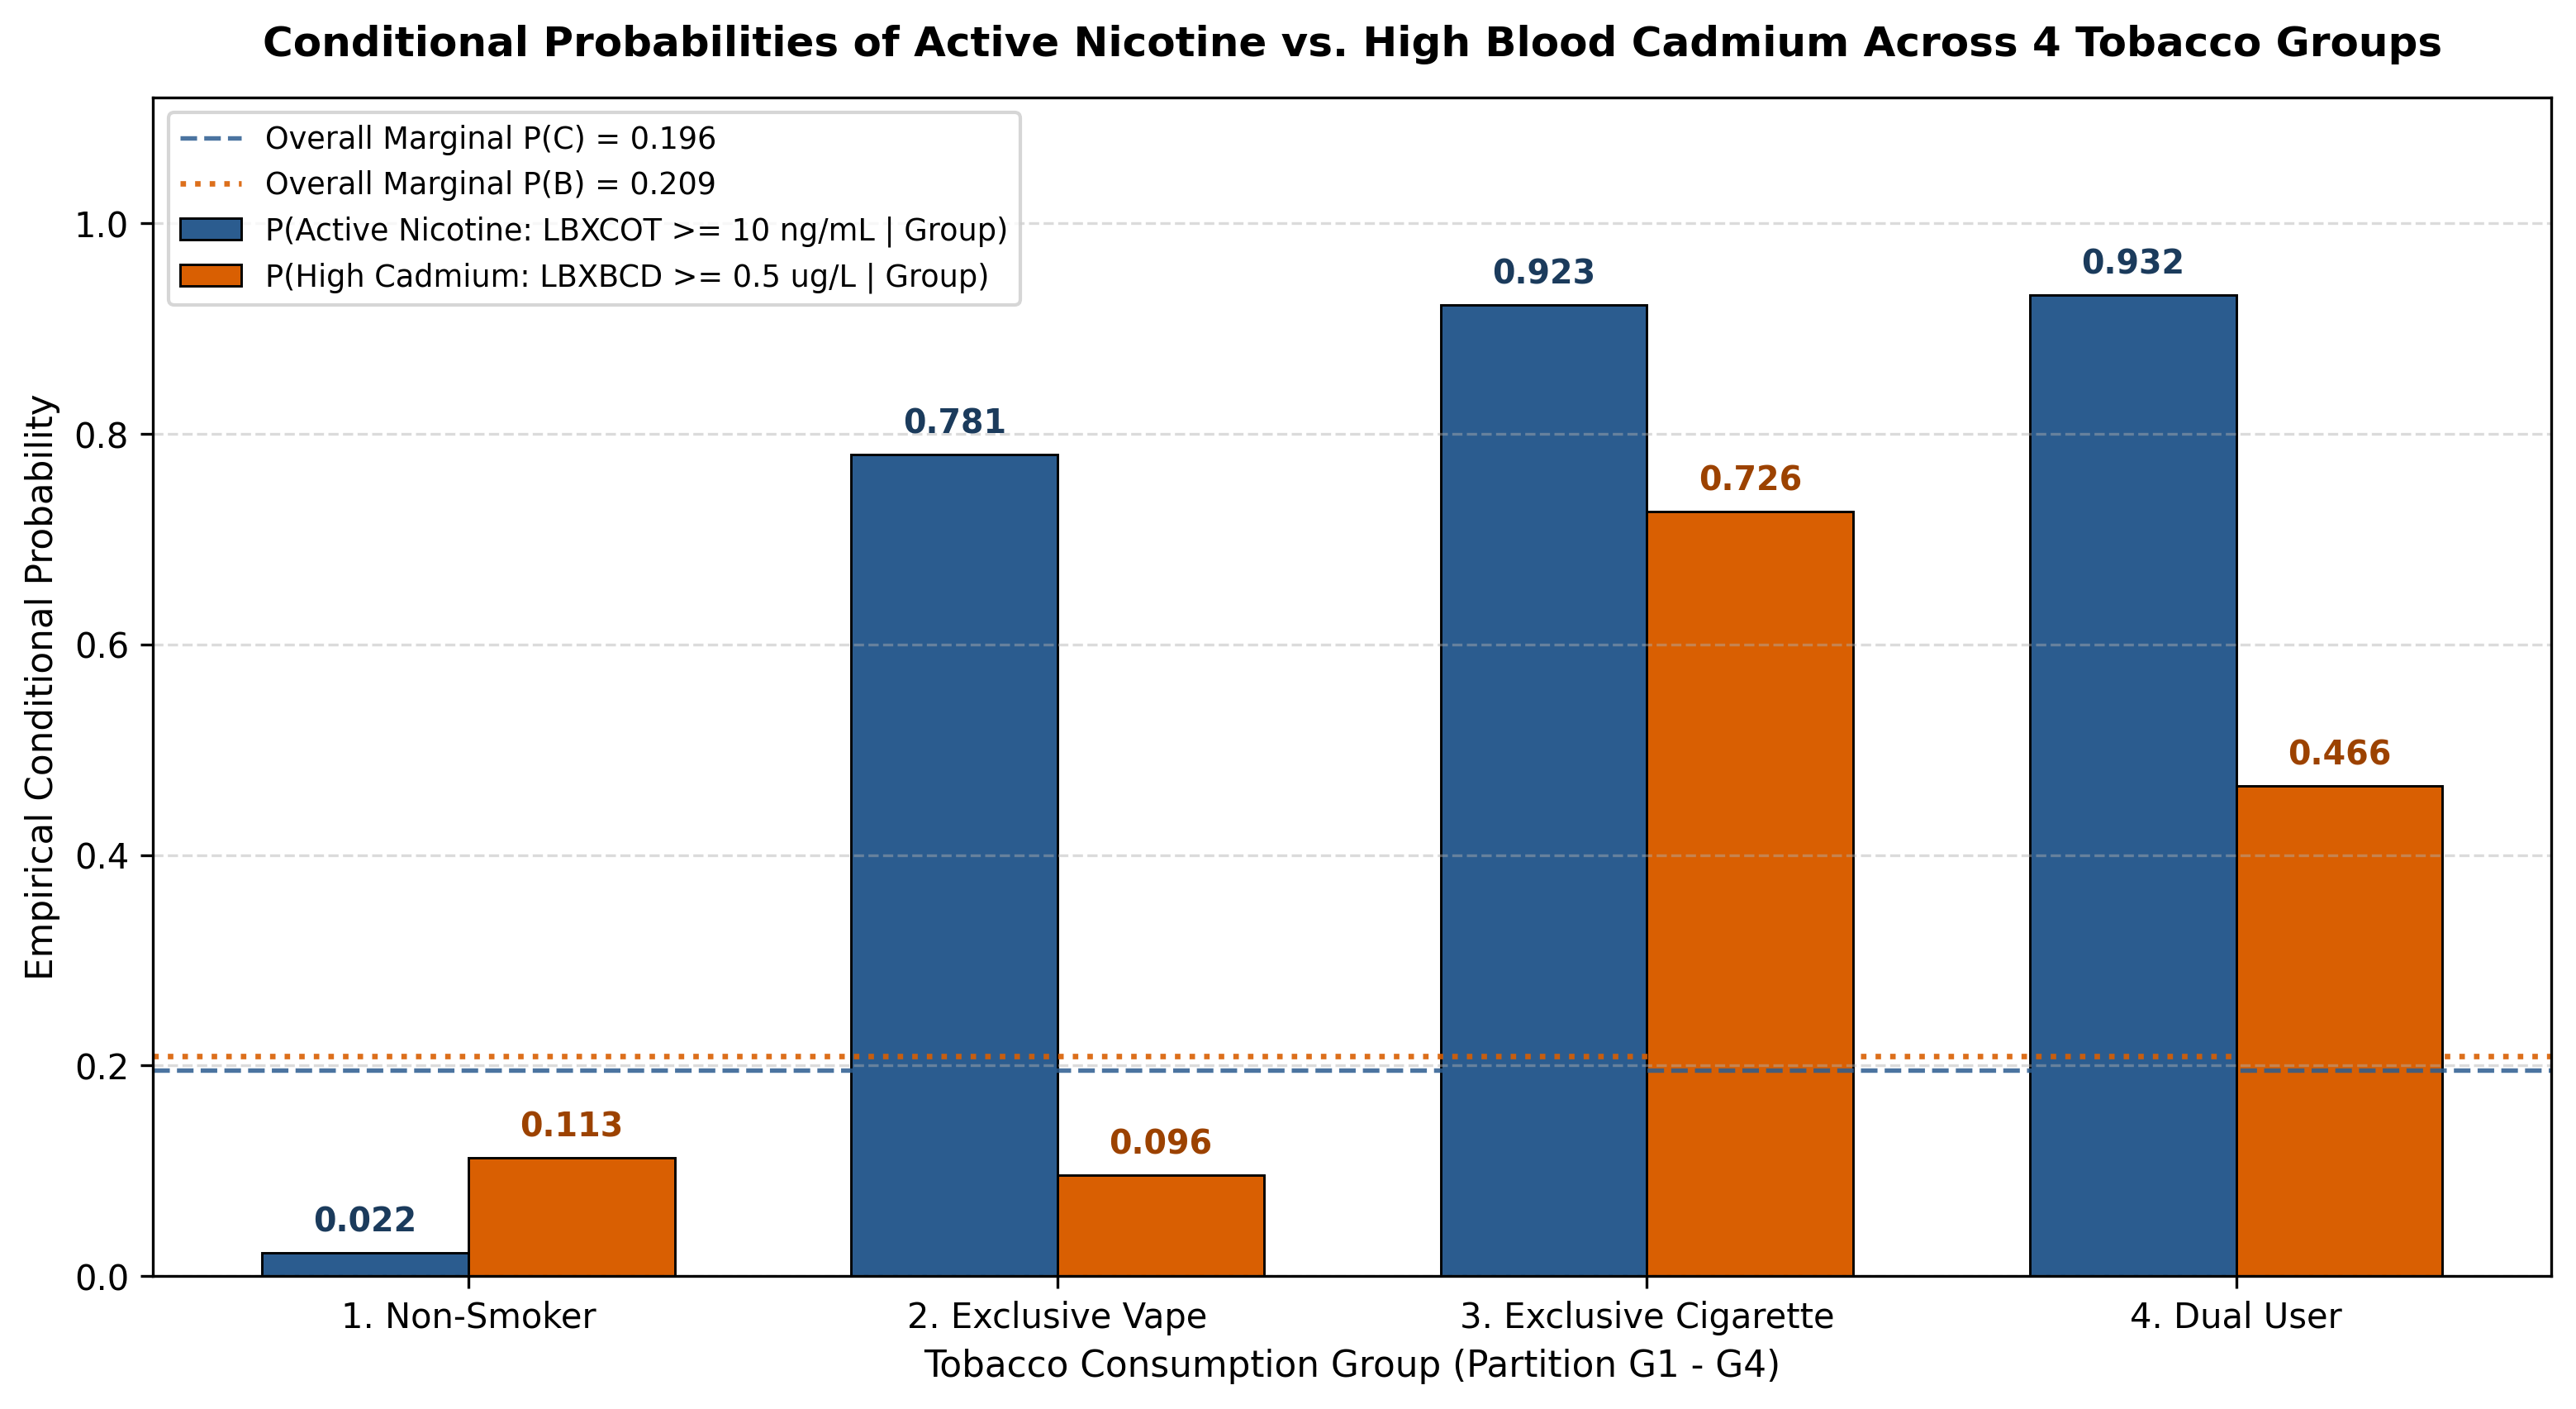
\includegraphics[width=0.76\textwidth]{figures/p2_fig1_conditional_probs.png}
\caption{مقایسه احتمال‌های شرطی مواجهه فعال با نیکوتین ($C$) و کادمیوم بالای خون ($B$) در چهار گروه مصرف دخانیات در برابر خطوط احتمال حاشیه‌ای کل جمعیت تحلیلی.}
\end{figure}


\section{بررسی مفهوم استقلال}

دو رویداد $E_1$ و $E_2$ از نظر آماری مستقل (\lr{Independent}) هستند اگر شرط‌گذاری روی یکی هیچ تغییری در احتمال وقوع دیگری ایجاد نکند ($P(E_2 \mid E_1) = P(E_2)$) و به طور معادل قاعده ضرب $P(E_1 \cap E_2) = P(E_1) \cdot P(E_2)$ برقرار باشد. بدون اجرای آزمون فرض رسمی، سازگاری داده‌ها با فرض استقلال را از طریق مقایسه مستقیم این دو معیار برای سه جفت رویداد ارزیابی می‌کنیم.

\begin{table}[htbp]
\centering
\caption{ارزیابی استدلالی استقلال رویدادها از طریق مقایسه $P(E_1 \cap E_2)$ با $P(E_1)\cdot P(E_2)$ در جمعیت تحلیلی (\lr{$N = 4,655$})}
\resizebox{\textwidth}{!}{
\begin{tabular}{llllllllll}
\toprule
جفت رویداد مورد بررسی & $P(E_1)$ & $P(E_2)$ & مشاهده‌شده $P(E_1 \cap E_2)$ & مورد انتظار $P(E_1)P(E_2)$ & اختلاف مشترک & نسبت مشاهده به انتظار & $P(E_2 \mid E_1)$ & $P(E_2 \mid E_1^c)$ & تغییر شرطی \\
\midrule
جفت ۱: سیگار احتراقی ($A$) و کادمیوم بالا ($B$) & \lr{0.1665} & \lr{0.2086} & \lr{0.1151} & \lr{0.0347} & \lr{+0.0804} & \lr{3.32} & \lr{0.6916} & \lr{0.1121} & \lr{+0.4830} \\
جفت ۲: سیگار احتراقی ($A$) و نیکوتین فعال ($C$) & \lr{0.1665} & \lr{0.1959} & \lr{0.1538} & \lr{0.0326} & \lr{+0.1212} & \lr{4.72} & \lr{0.9239} & \lr{0.0505} & \lr{+0.7280} \\
جفت ۳ (شاهد): جنسیت مرد ($M$) و کادمیوم بالا ($B$) & \lr{0.4498} & \lr{0.2086} & \lr{0.0782} & \lr{0.0938} & \lr{-0.0156} & \lr{0.83} & \lr{0.1738} & \lr{0.2370} & \lr{-0.0348} \\
\bottomrule
\end{tabular}
}
\end{table}

برای جفت اول یعنی مصرف سیگار احتراقی ($A$) و کادمیوم بالا ($B$)، تحت فرض استقلال باید احتمال مشترک برابر با $0.1665 \times 0.2086 = \text{\lr{0.0347}}$ (حدود \lr{162} نفر) می‌بود، اما مقدار مشاهده‌شده برابر با \lr{0.1151} (\lr{536} نفر و \lr{3.32} برابر انتظار) و اختلاف $P(B \mid A)$ از $P(B \mid A^c)$ برابر با \lr{57.95} واحد درصد است. در جفت دوم یعنی سیگار احتراقی ($A$) و نیکوتین فعال ($C$)، نقض استقلال حتی شدیدتر است (مشاهده‌شده \lr{0.1538} در برابر \lr{0.0326} مورد انتظار؛ \lr{4.72} برابر و جابه‌جایی شرطی \lr{+0.7280}). بنابراین داده‌ها برای هر دو جفت به وضوح با فرض استقلال ناسازگار بوده و نشانگر وابستگی مثبت بسیار نیرومند هستند.

برای مقایسه مقیاس وابستگی، جفت شاهد جنسیت مرد ($M$) و کادمیوم بالا ($B$) بررسی شد. احتمال مشترک مشاهده‌شده (\lr{0.0782}) به مقدار مورد انتظار تحت استقلال (\lr{0.0938}) بسیار نزدیک‌تر است (اختلاف \lr{-0.0156} و نسبت \lr{0.83})، اما همچنان برابر با صفر نیست و یک وابستگی منفی خفیف را نشان می‌دهد؛ به طوری که احتمال کادمیوم بالا در زنان (\lr{0.2370}) حدود \lr{6.32} واحد درصد بیشتر از مردان (\lr{0.1738}) است. این مشاهده با مکانیسم شناخته‌شده سم‌شناسی نیز همخوانی دارد که ذخایر آهن پایین‌تر در زنان موجب فعال‌تر شدن ناقل‌های جذب روده‌ای آهن و جذب هم‌زمان بیشتر کادمیوم می‌شود. بررسی رسمی معناداری این تفاوت‌ها به فازهای سوم و چهارم موکول می‌گردد.


\section{توزیع گسسته و مدل دوجمله‌ای}

متغیر تصادفی گسسته $K_{30}$ را به عنوان تعداد افراد دارای کادمیوم بالای خون ($B$: \lr{LBXBCD $\ge 0.5$}) در یک نمونه به اندازه ثابت \lr{$n = 30$} بزرگسال تعریف می‌کنیم (با احتمال تجربی کل $\hat{p} = \text{\lr{0.2086}}$). جدول زیر مشخصات مدل $\text{Binomial}(n=30, \hat{p})$ را در کنار واریانس دقیق بدون جایگذاری (مدل فوق‌هندسی با ضریب تصحیح $\frac{N-n}{N-1}$) در کل جمعیت تحلیلی و چهار گروه مصرف مقایسه می‌کند.

\begin{table}[htbp]
\centering
\caption{مشخصات مدل $\text{Binomial}(n=30, \hat{p})$ برای شمارش کادمیوم بالا ($B$) و مقایسه واریانس با مدل فوق‌هندسی}
\resizebox{\textwidth}{!}{
\begin{tabular}{lllllllllll}
\toprule
رژیم / زیرجمعیت هدف & حجم ($N$) & کسر $n/N$ & $\hat{p} = P(B)$ & $E[K_{30}]$ & واریانس دوجمله‌ای & واریانس فوق‌هندسی & \lr{SD} & $P(K=0)$ & $P(K \le 5)$ & $P(K \ge 10)$ \\
\midrule
کل جمعیت تحلیلی ($\Omega$) & \lr{4,655} & \lr{0.64\%} & \lr{0.2086} & \lr{6.26} & \lr{4.95} & \lr{4.92} & \lr{2.23} & \lr{0.0009} & \lr{0.3823} & \lr{0.0777} \\
\lr{1. Non-Smoker} ($G_1$) & \lr{3,734} & \lr{0.80\%} & \lr{0.1127} & \lr{3.38} & \lr{3.00} & \lr{2.98} & \lr{1.73} & \lr{0.0276} & \lr{0.8852} & \lr{0.0012} \\
\lr{2. Exclusive Vape} ($G_2$) & \lr{146} & \lr{20.55\%} & \lr{0.0959} & \lr{2.88} & \lr{2.60} & \lr{2.08} & \lr{1.61} & \lr{0.0486} & \lr{0.9379} & \lr{0.0003} \\
\lr{3. Exclusive Cigarette} ($G_3$) & \lr{672} & \lr{4.46\%} & \lr{0.7262} & \lr{21.79} & \lr{5.97} & \lr{5.71} & \lr{2.44} & \lr{0.0000} & \lr{0.0000} & \lr{1.0000} \\
\lr{4. Dual User} ($G_4$) & \lr{103} & \lr{29.13\%} & \lr{0.4660} & \lr{13.98} & \lr{7.47} & \lr{5.34} & \lr{2.73} & \lr{0.0000} & \lr{0.0006} & \lr{0.9511} \\
\bottomrule
\end{tabular}
}
\end{table}

در یک نمونه \lr{30} نفری از کل جمعیت تحلیلی (پنل \lr{A} شکل \lr{2})، به طور میانگین \lr{6.26} نفر کادمیوم بالا دارند و احتمال مشاهده \lr{10} نفر یا بیشتر \lr{0.0777} است. در گروه انحصاری ویپ میانگین به \lr{2.88} نفر افت کرده و احتمال مشاهده \lr{5} نفر یا کمتر به \lr{0.9379} می‌رسد، اما در سیگاری‌های سنتی میانگین برابر با \lr{21.79} نفر و احتمال مشاهده حداقل \lr{10} نفر عملاً برابر با \lr{1.0000} است.

\subsection{ارزیابی فرض‌های مدل دوجمله‌ای در داده‌های \lr{NHANES}}
از میان چهار فرض مدل دوجمله‌ای، ثابت بودن تعداد آزمایش‌ها ($n=30$) و دودویی بودن برآمد ($B/B^c$) دقیقاً برقرارند، اما دو فرض ثبات احتمال موفقیت ($p$) و استقلال آزمایش‌ها به سه دلیل ساختاری زیر نقض می‌شوند:

اول، نمونه‌گیری بدون جایگذاری از جامعه متناهی است که توزیع دقیق آن فوق‌هندسی (\lr{Hypergeometric}) است. تا زمانی که کسر نمونه‌گیری کوچک باشد ($n/N < \text{\lr{5\%}}$ تا \lr{10\%})، تقریب دوجمله‌ای کاملاً معقول است؛ چنان‌که برای کل نمونه (\lr{0.64\%})، غیرسیگاری‌ها (\lr{0.80\%}) و سیگاری‌های سنتی (\lr{4.46\%}) واریانس دوجمله‌ای و فوق‌هندسی تقریباً یکسان‌اند. اما در دو گروه کوچک انحصاری ویپ ($n/N = \text{\lr{20.55\%}}$) و مصرف دوگانه ($n/N = \text{\lr{29.13\%}}$)، واریانس فوق‌هندسی به ترتیب \lr{20\%} و \lr{28.5\%} کوچک‌تر است و تقریب دوجمله‌ای پراکندگی شمارش را بیش‌برآورد می‌کند.

دوم، ناهمگنی شدید احتمال $p$ میان زیرگروه‌های جمعیتی است؛ زیرا احتمال $P(B)$ بسته به نوع مصرف دخانیات از \lr{0.0959} تا \lr{0.7262} (و نیز بر حسب سن) تغییر می‌کند. بنابراین تقریب دوجمله‌ای تنها برای نمونه‌گیری تصادفی از کل چارچوب (با احتمال حاشیه‌ای واحد $\bar{p}$) یا از درون یک زیرجمعیت همگن و به اندازه کافی بزرگ معتبر است.

سوم، ساختار خوشه‌ای پیمایش \lr{NHANES} است. ممیزی \lr{30} واحد نمونه‌گیری اولیه (\lr{PSU}) نشان داد (پنل \lr{B} شکل \lr{2}) که نسبت تجربی $P(B)$ میان شهرستان‌ها از کمینه \lr{0.1382} تا بیشینه \lr{0.3333} (دامنه \lr{0.1951} و انحراف معیار \lr{0.0516}) نوسان دارد. شباهت محیطی و رفتاری افراد درون یک خوشه یا خانوار موجب همبستگی درون‌خوشه‌ای و نقض استقلال می‌شود و در نتیجه، در نمونه‌گیری‌های خوشه‌ای واقعی واریانس شمارش از $np(1-p)$ فراتر می‌رود.

\begin{figure}[htbp]
\centering
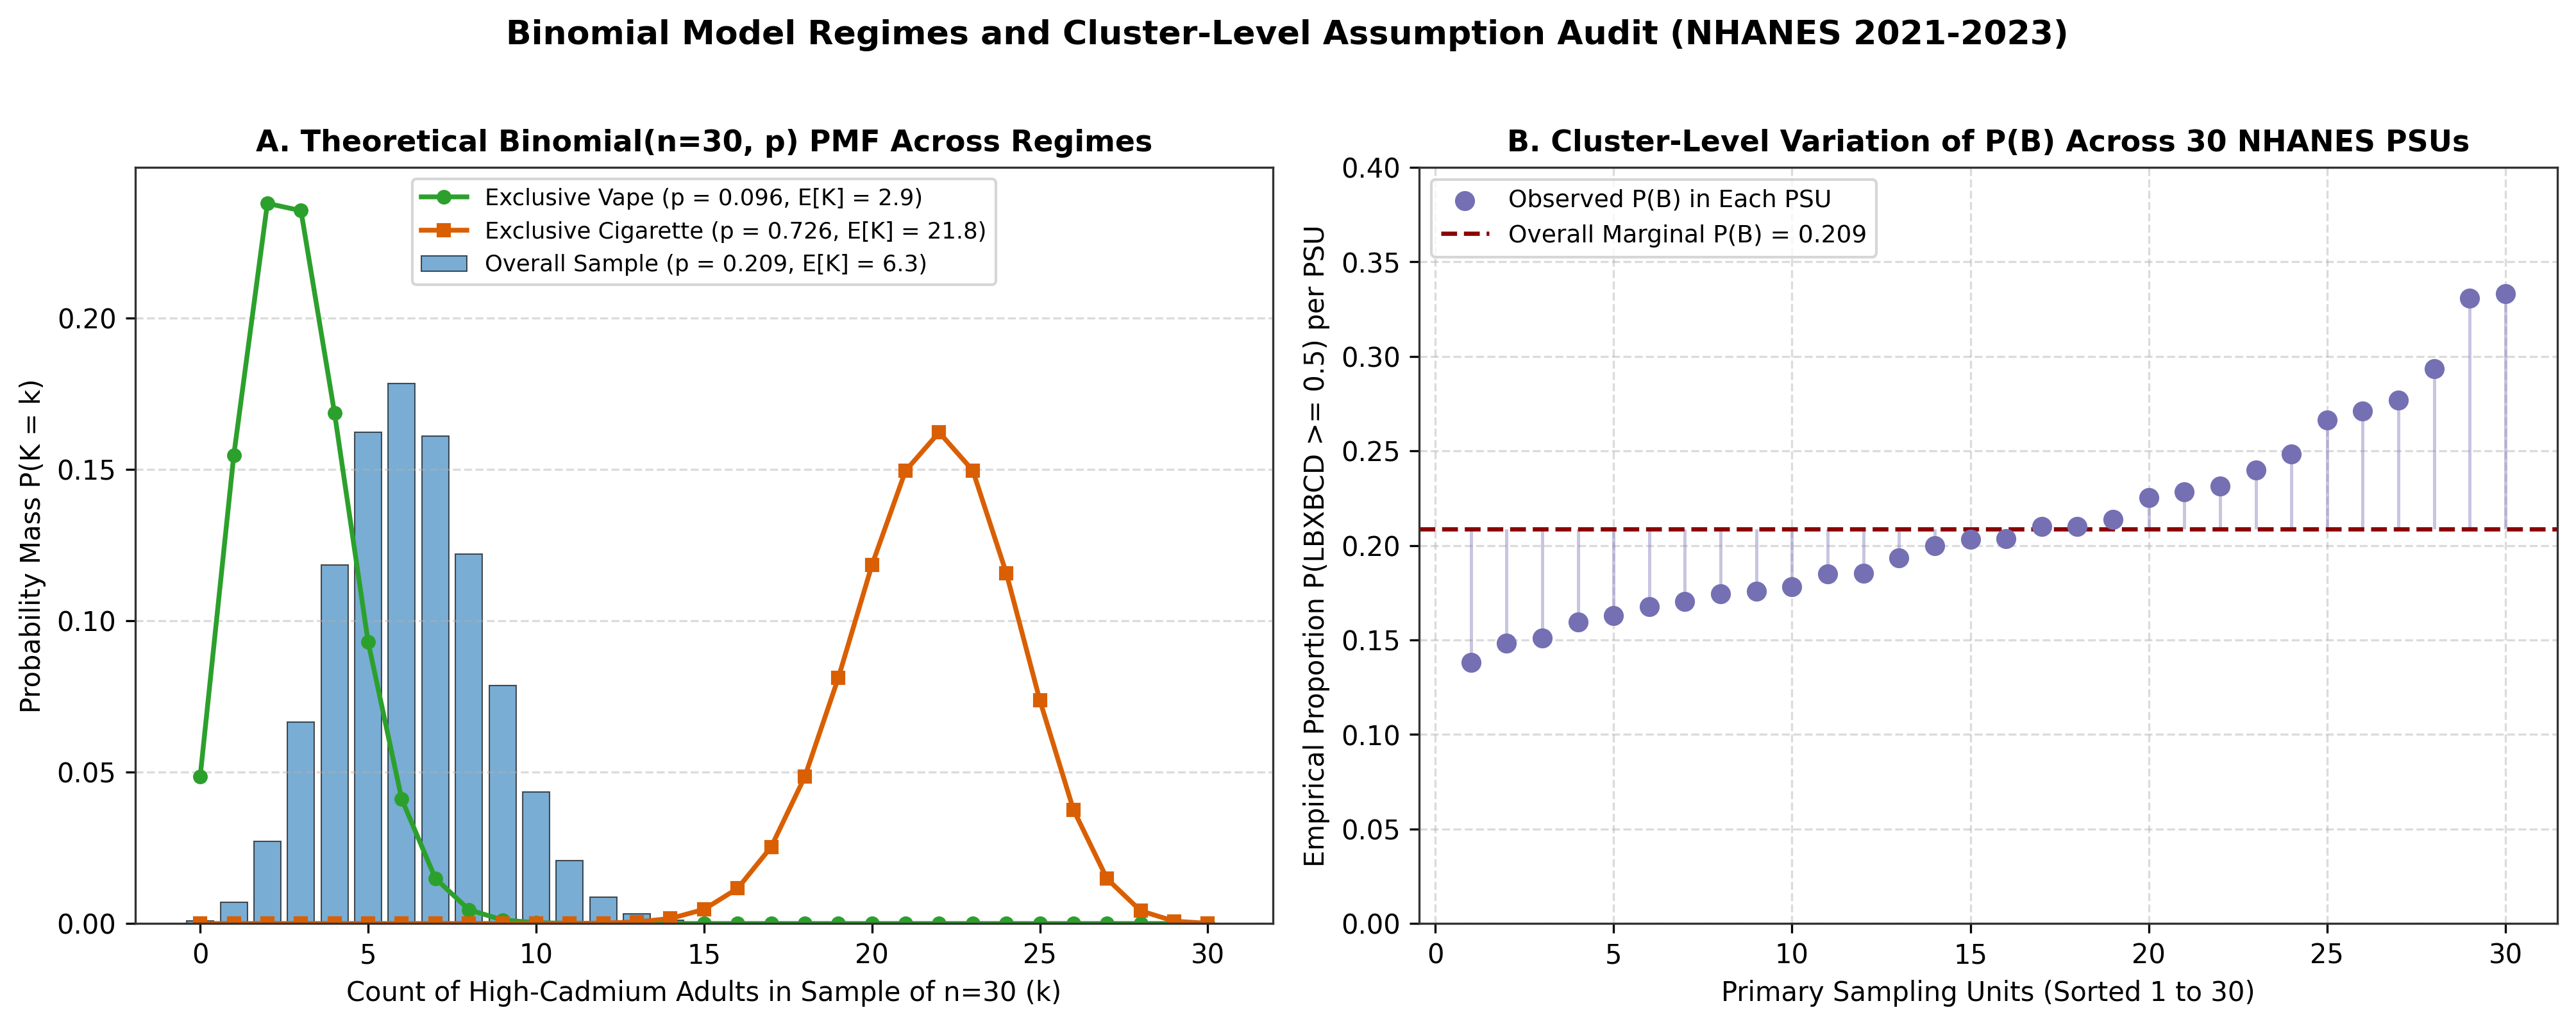
\includegraphics[width=0.80\textwidth]{figures/p2_fig2_binomial_model.png}
\caption{تابع جرم احتمال مدل $\text{Binomial}(30, p)$ در رژیم‌های مختلف مصرف دخانیات (الف) و پراکندگی نسبت تجربی کادمیوم بالا در میان \lr{30} خوشه جغرافیایی \lr{NHANES} (ب).}
\end{figure}


\section{متغیر پیوسته و تقریب توزیع نرمال}

برای ارزیابی جامع تقریب نرمال بدون اتکا به صرف یک عدد آزمون، غلظت کادمیوم خون را در دو مقیاس خام ($W = \text{LBXBCD}$) و لگاریتمی ($Y_1 = \log_{10}(\text{LBXBCD})$) بر روی جمعیت تحلیلی (\lr{$N = 4,655$}) از طریق شاخص‌های شکل، قانون تجربی \lr{68-95-99.7\%}، مقایسه صدک‌ها، هیستوگرام و نمودار \lr{Q-Q} بررسی می‌کنیم.

\begin{table}[htbp]
\centering
\caption{مقایسه شاخص‌های شکل، قانون تجربی \lr{68-95-99.7\%} و احتمال منفی ناممکن برای کادمیوم خام و لگاریتمی}
\resizebox{\textwidth}{!}{
\begin{tabular}{lllllllllll}
\toprule
متغیر پیوسته & $N$ & میانگین & میانه & \lr{SD} & چولگی & کشیدگی مازاد & درون $1\text{SD}$ & درون $2\text{SD}$ & درون $3\text{SD}$ & $P_{\text{norm}}(X < 0)$ \\
 & & & & & & (نرمال: \lr{0}) & (نرمال: \lr{68.27\%}) & (نرمال: \lr{95.45\%}) & (نرمال: \lr{99.73\%}) & \\
\midrule
$W$: کادمیوم خام (\lr{ug/L}) & \lr{4,655} & \lr{0.4076} & \lr{0.2620} & \lr{0.5005} & \lr{5.251} & \lr{42.570} & \lr{92.03\%} & \lr{96.24\%} & \lr{98.13\%} & \lr{20.77\%} \\
$Y_1$: $\log_{10}(\text{LBXBCD})$ & \lr{4,655} & \lr{-0.5424} & \lr{-0.5817} & \lr{0.3325} & \lr{0.670} & \lr{0.717} & \lr{70.91\%} & \lr{95.15\%} & \lr{99.25\%} & ندارد \\
\bottomrule
\end{tabular}
}
\end{table}

\begin{table}[htbp]
\centering
\caption{مقایسه پنج صدک تجربی کلیدی با صدک‌های نظری توزیع نرمال $N(\hat{\mu}, \hat{\sigma}^2)$ برای $W$ و $Y_1$}
\resizebox{0.92\textwidth}{!}{
\begin{tabular}{l|llll|llll}
\toprule
صدک & \multicolumn{4}{c|}{کادمیوم خام ($W = \text{LBXBCD}$)} & \multicolumn{4}{c}{کادمیوم لگاریتمی ($Y_1 = \log_{10}(\text{LBXBCD})$)} \\
 & تجربی & نظری نرمال & اختلاف & وضعیت برازش & تجربی & نظری نرمال & اختلاف & وضعیت برازش \\
\midrule
\lr{P5} & \lr{0.0960} & \lr{-0.4156} & \lr{+0.5116} & غیرممکن (منفی) & \lr{-1.0177} & \lr{-1.0892} & \lr{+0.0715} & نزدیک \\
\lr{P25} & \lr{0.1700} & \lr{0.0701} & \lr{+0.0999} & انحراف زیاد & \lr{-0.7696} & \lr{-0.7666} & \lr{-0.0029} & تقریباً منطبق \\
\lr{P50} & \lr{0.2620} & \lr{0.4076} & \lr{-0.1456} & چولگی شدید & \lr{-0.5817} & \lr{-0.5424} & \lr{-0.0393} & نزدیک \\
\lr{P75} & \lr{0.4420} & \lr{0.7452} & \lr{-0.3032} & انحراف شدید & \lr{-0.3546} & \lr{-0.3181} & \lr{-0.0364} & نزدیک \\
\lr{P95} & \lr{1.2203} & \lr{1.2309} & \lr{-0.0106} & تصادفی & \lr{0.0865} & \lr{0.0045} & \lr{+0.0820} & دنباله راست خفیف \\
\bottomrule
\end{tabular}
}
\end{table}

داده‌های جدول‌های بالا و پنل‌های \lr{A} و \lr{B} شکل \lr{3} نشان می‌دهند که تقریب نرمال برای کادمیوم خام ($W$) کاملاً نامناسب است: چولگی (\lr{5.251}) و کشیدگی مازاد (\lr{42.570}) بسیار شدید بوده، قانون تجربی به کلی نقض می‌شود (\lr{92.03\%} مشاهدات درون $1\text{SD}$ به جای \lr{68.27\%} و \lr{1.87\%} بیرون از $3\text{SD}$)، و از آنجا که میانگین (\lr{0.4076}) کوچک‌تر از انحراف معیار (\lr{0.5005}) است، مدل نرمال برازش‌شده دقیقاً \lr{20.77\%} از کل احتمال را به مقادیر منفی و غیرممکن اختصاص می‌دهد (صدک پنجم نظری \lr{-0.4156 ug/L}). در نمودار \lr{Q-Q} (پنل \lr{B}) نیز انحنای شدید از خط مرجع کاملاً مشهود است.

با اعمال تبدیل لگاریتمی ($Y_1$، پنل‌های \lr{C} و \lr{D})، چولگی به \lr{0.670} و کشیدگی به \lr{0.717} افت کرده و انطباق با قانون تجربی (\lr{70.91\%}، \lr{95.15\%} و \lr{99.25\%}) و صدک‌های میانی بسیار خوب می‌شود. در نمودار \lr{Q-Q} پنل \lr{D} تنها دو انحراف جزئی اما بامعنا در انتهاها باقی می‌ماند: یک پله افقی در انتهای چپ ($z < -2.4$ روی \lr{-1.337}) ناشی از سانسور زیر حد تشخیص آزمایشگاه ($\log_{10}(0.046)$)، و خمیدگی خفیف رو به بالا در انتهای راست ($z > +1.5$) ناشی از حضور سیگاری‌های قهار در این توزیع مخلوط. بنابراین تقریب نرمال برای $Y_1$ در بدنه اصلی کاملاً معقول بوده و پایه استفاده از آن در مدل‌های پارامتریک فازهای بعدی است.

\begin{figure}[htbp]
\centering
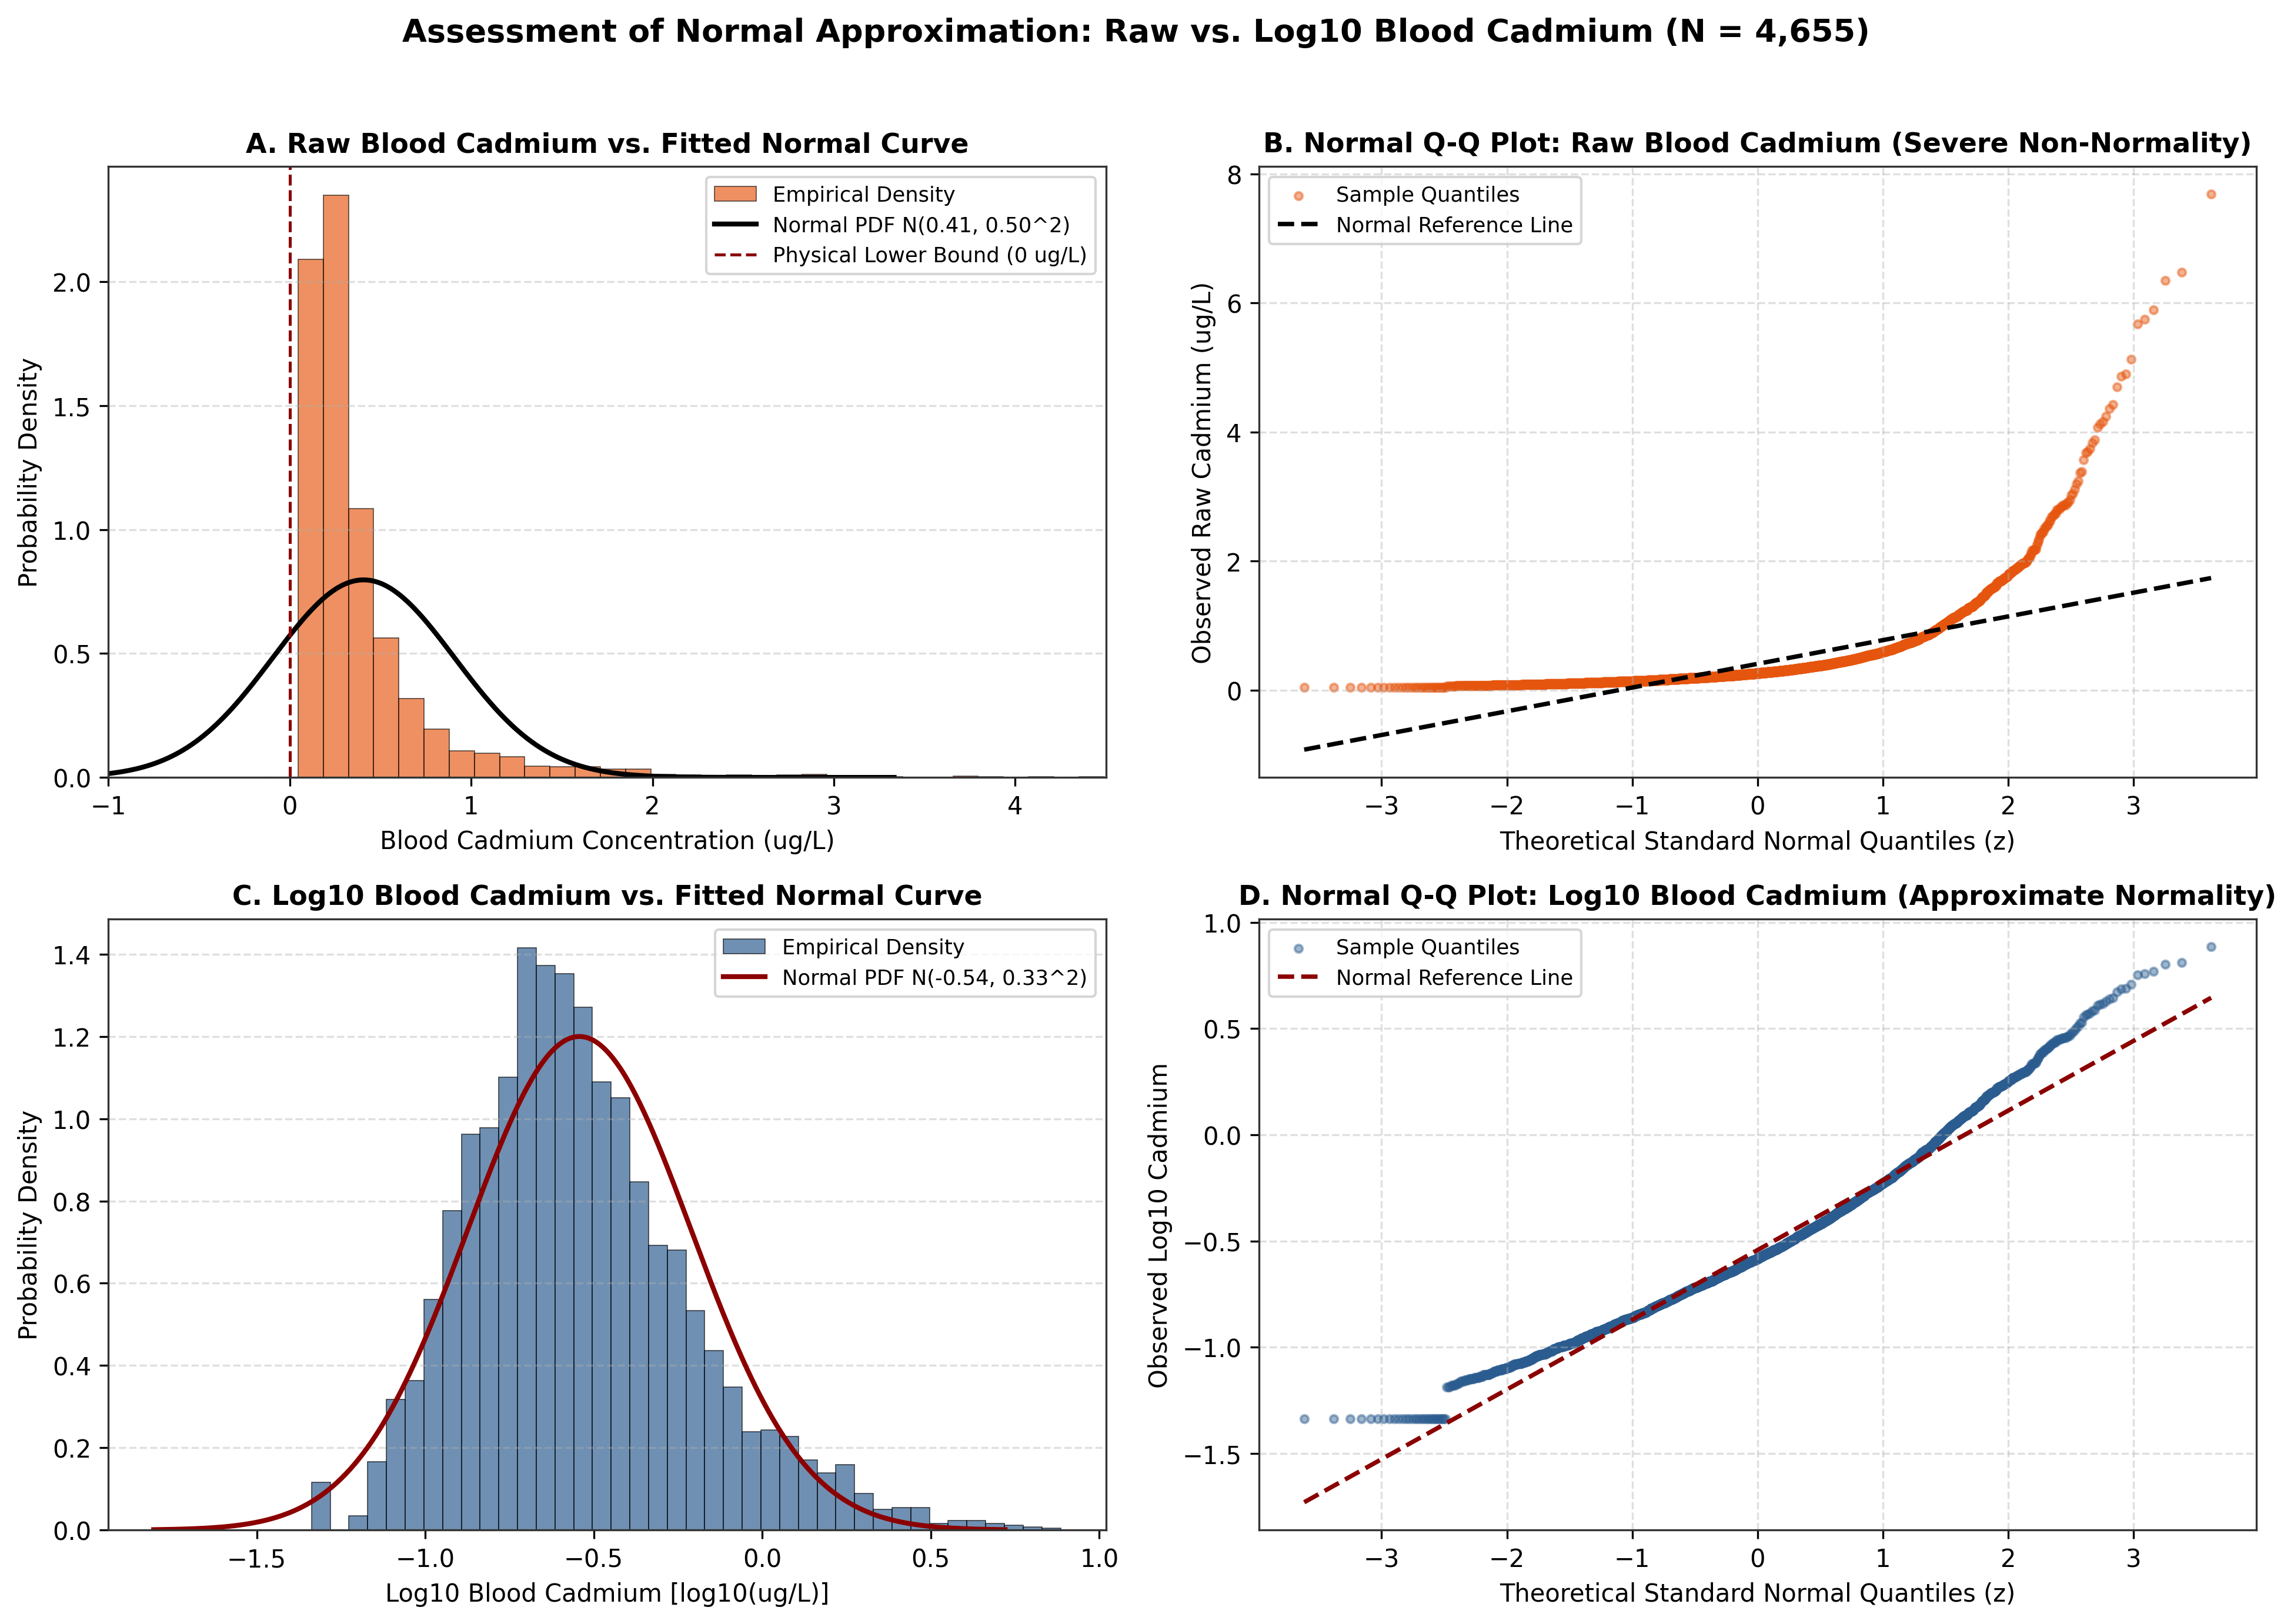
\includegraphics[width=0.74\textwidth]{figures/p2_fig3_normality_cadmium.png}
\caption{ارزیابی تقریب توزیع نرمال برای کادمیوم خون در مقیاس خام (پنل‌های \lr{A} و \lr{B}) در برابر مقیاس تبدیل‌یافته لگاریتمی پایه \lr{10} (پنل‌های \lr{C} و \lr{D}).}
\end{figure}


\section{امید ریاضی و واریانس}

برای نمایش صریح محاسبه امید ریاضی ($\mu = \sum x p(x)$) و واریانس ($\sigma^2 = \sum (x - \mu)^2 p(x)$) از یک توزیع احتمال تجربی گسسته، ابتدا متغیر تعداد روزهای مصرف سیگار در \lr{5} روز گذشته ($D_{\text{cig}} = \text{SMQ710}$) را در میان \lr{633} مصرف‌کننده فعال سیگار کاغذی بررسی می‌کنیم (کمتر بودن این عدد از \lr{775} سیگاری احتراقی به دلیل وجود مصرف‌کنندگان صرفاً پیپ/سیگار برگ یا سیگاری‌های غیرفعال در \lr{5} روز اخیر است).

\begin{table}[htbp]
\centering
\caption{محاسبه گام‌به‌گام امید ریاضی و واریانس از توزیع احتمال تجربی تعداد روز مصرف سیگار ($D_{\text{cig}}$، \lr{$N = 633$})}
\resizebox{0.88\textwidth}{!}{
\begin{tabular}{lllll}
\toprule
تعداد روز مصرف ($x$) & فراوانی ($n$) & احتمال تجربی $p(x)$ & سهم در امید $x \cdot p(x)$ & سهم در واریانس $(x - E[X])^2 p(x)$ \\
\midrule
\lr{1} روز & \lr{24} & \lr{0.0379} & \lr{0.0379} & \lr{0.4672} \\
\lr{2} روز & \lr{36} & \lr{0.0569} & \lr{0.1137} & \lr{0.3584} \\
\lr{3} روز & \lr{33} & \lr{0.0521} & \lr{0.1564} & \lr{0.1189} \\
\lr{4} روز & \lr{40} & \lr{0.0632} & \lr{0.2528} & \lr{0.0165} \\
\lr{5} روز (هر روز) & \lr{500} & \lr{0.7899} & \lr{3.9494} & \lr{0.1894} \\
\midrule
مجموع کل & \lr{633} & \lr{1.0000} & $E[D_{\text{cig}}] = \text{\lr{4.5103}}$ & $\text{Var}(D_{\text{cig}}) = \text{\lr{1.1504}}$ \\
\bottomrule
\end{tabular}
}
\end{table}

همان‌طور که جدول نشان می‌دهد، \lr{78.99\%} سیگاری‌های فعال در تمامی \lr{5} روز گذشته سیگار کشیده‌اند که امید ریاضی بالای \lr{4.5103} روز در بازه \lr{5} روزه اخیر را ایجاد می‌کند و گویای وابستگی روزانه به نیکوتین است. واریانس \lr{1.1504} (انحراف معیار \lr{1.0726} روز) نیز عمدتاً ناشی از اقلیت حدود \lr{15\%} سیگاری‌های غیرروزانه ($x \in \{1, 2, 3\}$) است.

جدول زیر مقادیر امید ریاضی، واریانس تجربی، واریانس نمونه‌ای و انحراف معیار تجربی تمامی متغیرهای گسسته و پیوسته اصلی فاز دوم را گزارش می‌کند.

\begin{table}[htbp]
\centering
\caption{امید ریاضی، واریانس تجربی، واریانس نمونه‌ای و انحراف معیار تجربی متغیرهای تصادفی گسسته و پیوسته}
\resizebox{\textwidth}{!}{
\begin{tabular}{lllllll}
\toprule
متغیر تصادفی & نوع تکیه‌گاه & تعداد معتبر & $E[X]$ & واریانس تجربی & واریانس نمونه‌ای & انحراف معیار تجربی \\
\midrule
$X_B$: نشانگر کادمیوم بالا & گسسته $\{0, 1\}$ & \lr{4,655} & \lr{0.2086} & \lr{0.1651} & \lr{0.1651} & \lr{0.4063} \\
$X_C$: نشانگر نیکوتین فعال & گسسته $\{0, 1\}$ & \lr{4,655} & \lr{0.1959} & \lr{0.1575} & \lr{0.1576} & \lr{0.3969} \\
$D_{\text{cig}}$: روزهای سیگار (\lr{SMQ710}) & گسسته $\{1, \dots, 5\}$ & \lr{633} & \lr{4.5103} & \lr{1.1504} & \lr{1.1522} & \lr{1.0726} \\
$K_{30}$: شمارش $B$ در $n=30$ & گسسته $\{0, \dots, 30\}$ & مدل دوجمله‌ای & \lr{6.2578} & \lr{4.9525} & --- & \lr{2.2254} \\
$W$: کادمیوم خام (\lr{ug/L}) & پیوسته & \lr{4,655} & \lr{0.4076} & \lr{0.2504} & \lr{0.2505} & \lr{0.5004} \\
$Y_1$: $\log_{10}(\text{LBXBCD})$ & پیوسته & \lr{4,655} & \lr{-0.5424} & \lr{0.1105} & \lr{0.1105} & \lr{0.3324} \\
$Y_2$: $\log_{10}(\text{LBXCOT})$ & پیوسته & \lr{4,655} & \lr{-0.9899} & \lr{2.7952} & \lr{2.7958} & \lr{1.6719} \\
$Y_3$: هموگلوبین خون (\lr{g/dL}) & پیوسته & \lr{4,638} & \lr{13.9092} & \lr{2.1033} & \lr{2.1037} & \lr{1.4503} \\
\bottomrule
\end{tabular}
}
\end{table}

برای متغیرهای نشانگر $X_B$ و $X_C$، امید ریاضی برابر احتمال وقوع رویداد (\lr{0.2086} و \lr{0.1959}) و واریانس برابر $p(1-p)$ است. در شمارش $K_{30}$، میانگین مورد انتظار در نمونه‌های \lr{30} نفری برابر \lr{6.26} نفر با نوسان معمول \lr{2.23} نفر است. در متغیرهای پیوسته، هموگلوبین با امید \lr{13.9092 g/dL} و انحراف معیار محدود \lr{1.4503 g/dL} بیانگر ثبات فیزیولوژیک بالاست. در مقابل، واریانس بزرگ لگاریتم کوتینین (\lr{2.7952}) در برابر واریانس فشرده لگاریتم کادمیوم (\lr{0.1105}) بازتاب ساختار دووجهی شدید کوتینین میان غیرسیگاری‌ها و مصرف‌کنندگان است؛ همچنین با تبدیل معکوس امید ریاضی $Y_1$، میانگین هندسی کادمیوم خون برابر $10^{-0.5424} \approx \text{\lr{0.287 ug/L}}$ به دست می‌آید که بسیار نزدیک به میانه تجربی (\lr{0.262 ug/L}) است.


\section{دو متغیر تصادفی و کوواریانس}

برای بررسی جهت رابطه خطی هم‌زمان میان دو متغیر پیوسته بدون ورود به همبستگی رسمی و استنباط‌های فاز چهارم، کوواریانس $\text{Cov}(X, Y) = E[(X - \mu_X)(Y - \mu_Y)]$ و سهم مشاهدات در ربع‌های هم‌جهت ($Q_1 + Q_3$ با حاصل‌ضرب انحراف مثبت) در برابر ربع‌های خلاف‌جهت ($Q_2 + Q_4$ با حاصل‌ضرب منفی) پیرامون نقطه $(\bar{X}, \bar{Y})$ برای سه جفت متغیر کلیدی محاسبه شد.

\begin{table}[htbp]
\centering
\caption{کوواریانس تجربی، سهم ربع‌های هم‌جهت و خلاف‌جهت و جهت رابطه برای سه جفت متغیر پیوسته}
\resizebox{\textwidth}{!}{
\begin{tabular}{lllllllll}
\toprule
جفت متغیر پیوسته ($X$ و $Y$) & $N$ & $\bar{X}$ & $\bar{Y}$ & کوواریانس تجربی & کوواریانس نمونه‌ای & سهم $Q_1+Q_3$ (+) & سهم $Q_2+Q_4$ (-) & جهت رابطه \\
\midrule
جفت ۱: $\log_{10}(\text{LBXCOT})$ و $\log_{10}(\text{LBXBCD})$ & \lr{4,655} & \lr{-0.9899} & \lr{-0.5424} & \lr{+0.2769} & \lr{+0.2769} & \lr{64.64\%} & \lr{35.36\%} & مثبت (مستقیم) \\
جفت ۲: سن (\lr{RIDAGEYR}) و $\log_{10}(\text{LBXBCD})$ & \lr{4,655} & \lr{54.1334} & \lr{-0.5424} & \lr{+1.3916} & \lr{+1.3919} & \lr{59.36\%} & \lr{40.64\%} & مثبت (مستقیم) \\
جفت ۳: درآمد (\lr{INDFMPIR}) و $\log_{10}(\text{LBXBCD})$ & \lr{4,103} & \lr{3.0711} & \lr{-0.5376} & \lr{-0.1076} & \lr{-0.1076} & \lr{43.99\%} & \lr{56.01\%} & منفی (معکوس) \\
\bottomrule
\end{tabular}
}
\end{table}

در جفت اول (پنل \lr{A} شکل \lr{4})، کوواریانس مثبت (\lr{+0.2769}) و تمرکز \lr{64.64\%} مشاهدات در ربع‌های مثبت، همراهی مستقیم مواجهه با نیکوتین و کادمیوم را نشان می‌دهد؛ خوشه سمت چپ شامل ستون عمودی مقادیر زیر حد تشخیص کوتینین (\lr{-2.155}) در ربع سوم قرار دارد و مصرف‌کنندگان فعال نیکوتین به ربع اول کشیده شده‌اند، در حالی که نقاط پراکنده در ربع چهارم (نیکوتین بالا همراه با کادمیوم پایین) دقیقاً متناظر با مصرف‌کنندگان انحصاری ویپ هستند. در جفت دوم (پنل \lr{B})، کوواریانس مثبت سن با لگاریتم کادمیوم (\lr{+1.3919}) روند انباشت زیستی کادمیوم با افزایش سن را تایید می‌کند. در جفت سوم (پنل \lr{C}، روی \lr{4,103} فرد دارای درآمد معتبر)، کوواریانس منفی (\lr{-0.1076}) و سهم \lr{56.01\%} نقاط در ربع‌های منفی نشان‌دهنده کاهش سطح کادمیوم در سطوح بالاتر درآمد است (خط عمودی سمت راست روی \lr{5.0} ناشی از سانسور از بالای درآمد است).

نکته کلیدی در مقایسه جفت اول و دوم آن است که اگرچه عدد کوواریانس سن (\lr{+1.3919}) پنج برابر کوواریانس لگاریتم کوتینین (\lr{+0.2769}) است، نمی‌توان نتیجه گرفت رابطه سن قوی‌تر است؛ زیرا کوواریانس به شدت به واحد و مقیاس متغیرها وابسته است (انحراف معیار سن حدود \lr{17} سال در برابر \lr{1.67} واحد برای لگاریتم کوتینین). تمرکز بالاتر نقاط در ربع‌های هم‌جهت برای کوتینین (\lr{64.64\%} در برابر \lr{59.36\%}) نیز این موضوع را تایید می‌کند و مقایسه بی‌واحد شدت روابط از طریق ضریب همبستگی در فاز چهارم انجام خواهد شد.

\begin{figure}[htbp]
\centering
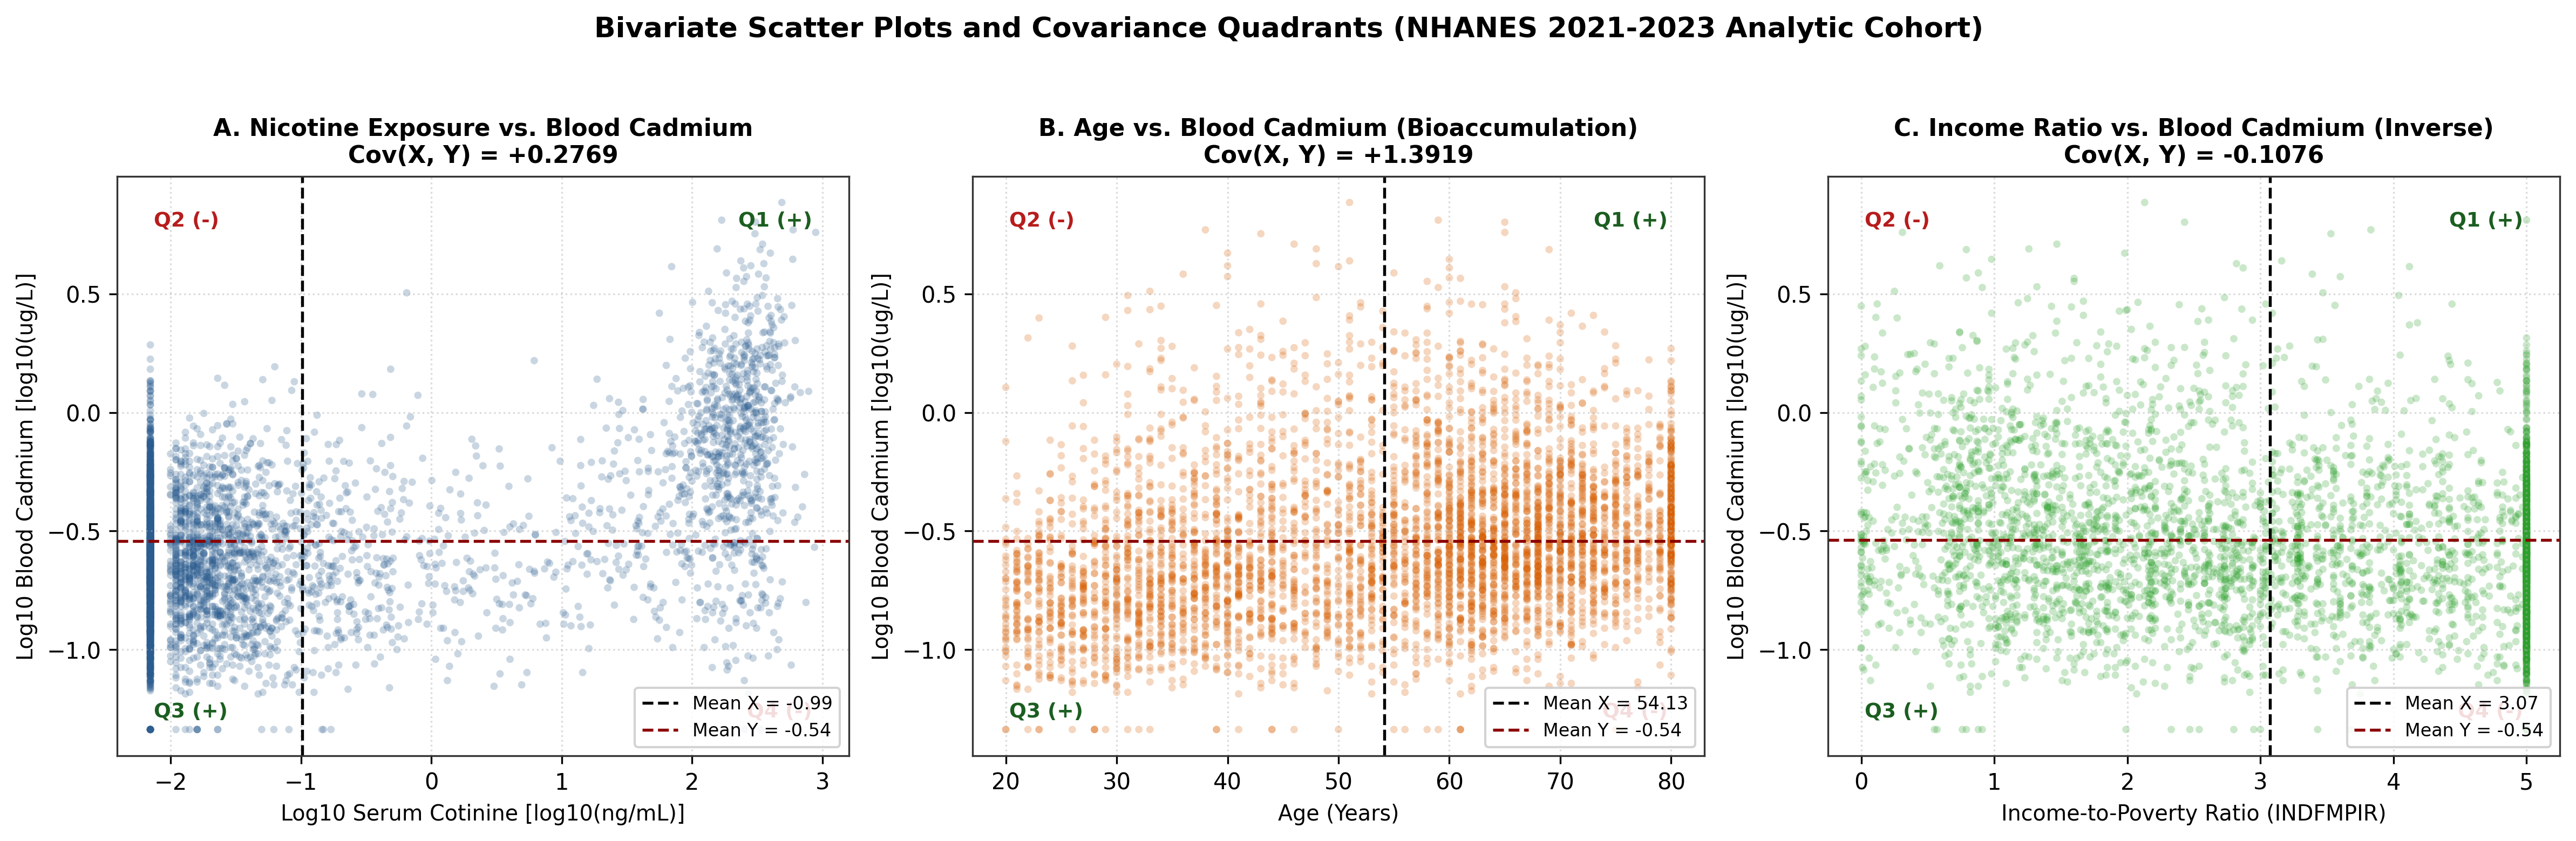
\includegraphics[width=0.90\textwidth]{figures/p2_fig4_bivariate_covariance.png}
\caption{نمودار پراکنش و ربع‌های کوواریانس برای رابطه لگاریتم کادمیوم خون با لگاریتم کوتینین سرم (الف)، سن (ب) و نسبت درآمد به خط فقر (ج).}
\end{figure}


\section{قضیه بیز و به‌روزرسانی تشخیصی احتمال}

ساختار این پژوهش برای به‌روزرسانی بیزی کاملاً مناسب است؛ زیرا می‌توان با مشاهده نتایج عینی آزمایش خون ($E$)، احتمال پیشین تعلق فرد به هر یک از چهار گروه افراز ($G_1$ تا $G_4$) را به احتمال پسین به‌روزرسانی کرد:
$$
P(G_i \mid E) = \frac{P(G_i) \, P(E \mid G_i)}{P(E)}, \qquad P(E) = \sum_{j=1}^{4} P(G_j) \, P(E \mid G_j)
$$
در جدول زیر، این به‌روزرسانی با فراوانی‌های تجربی جمعیت تحلیلی (\lr{$N = 4,655$}) تحت دو شواهد زیستی متفاوت اجرا شده است: سناریوی اول مشاهده کادمیوم بالا ($B$: \lr{LBXBCD $\ge 0.5$}) و سناریوی دوم مشاهده الگوی ترکیبی نیکوتین فعال همراه با کادمیوم پایین ($E_2 = C \cap B^c$).

\begin{table}[htbp]
\centering
\caption{به‌روزرسانی بیزی چهار گروه مصرف دخانیات تحت دو شواهد زیستی $B$ (کادمیوم بالا) و $E_2 = C \cap B^c$ (نیکوتین فعال و کادمیوم پایین)}
\resizebox{\textwidth}{!}{
\begin{tabular}{llllllll}
\toprule
فرضیه / گروه ($G_i$) & حجم گروه & پیشین $P(G_i)$ & درست‌نمایی $P(E \mid G_i)$ & مشترک $P(G_i \cap E)$ & کل $P(E)$ & پسین $P(G_i \mid E)$ & ضریب به‌روزرسانی \\
\midrule
\multicolumn{8}{c}{\textbf{سناریوی ۱: مشاهده کادمیوم بالای خون ($E = B$: \lr{LBXBCD $\ge 0.5$ ug/L})}} \\
\midrule
$G_1$: \lr{1. Non-Smoker} & \lr{3,734} & \lr{0.8021} & \lr{0.1127} & \lr{0.0904} & \lr{0.2086} & \lr{0.4336} & \lr{0.54} \\
$G_2$: \lr{2. Exclusive Vape} & \lr{146} & \lr{0.0314} & \lr{0.0959} & \lr{0.0030} & \lr{0.2086} & \lr{0.0144} & \lr{0.46} \\
$G_3$: \lr{3. Exclusive Cigarette} & \lr{672} & \lr{0.1444} & \lr{0.7262} & \lr{0.1048} & \lr{0.2086} & \lr{0.5026} & \lr{3.48} \\
$G_4$: \lr{4. Dual User} & \lr{103} & \lr{0.0221} & \lr{0.4660} & \lr{0.0103} & \lr{0.2086} & \lr{0.0494} & \lr{2.23} \\
\midrule
\multicolumn{8}{c}{\textbf{سناریوی ۲: مشاهده نیکوتین فعال همراه با کادمیوم پایین ($E_2 = C \cap B^c$)}} \\
\midrule
$G_1$: \lr{1. Non-Smoker} & \lr{3,734} & \lr{0.8021} & \lr{0.0142} & \lr{0.0114} & \lr{0.0739} & \lr{0.1541} & \lr{0.19} \\
$G_2$: \lr{2. Exclusive Vape} & \lr{146} & \lr{0.0314} & \lr{0.6986} & \lr{0.0219} & \lr{0.0739} & \lr{0.2965} & \lr{9.45} \\
$G_3$: \lr{3. Exclusive Cigarette} & \lr{672} & \lr{0.1444} & \lr{0.2098} & \lr{0.0303} & \lr{0.0739} & \lr{0.4099} & \lr{2.84} \\
$G_4$: \lr{4. Dual User} & \lr{103} & \lr{0.0221} & \lr{0.4660} & \lr{0.0103} & \lr{0.0739} & \lr{0.1395} & \lr{6.31} \\
\bottomrule
\end{tabular}
}
\end{table}

در سناریوی اول، با مشاهده کادمیوم بالا ترتیب احتمالات به کلی تغییر می‌کند: احتمال سیگار انحصاری با جهش \lr{3.48} برابری از \lr{0.1444} به \lr{0.5026} می‌رسد و به محتمل‌ترین گروه تبدیل می‌شود (در ترکیب دودویی نیز با قانون احتمال کل $P(B) = (0.1665)(0.6916) + (0.8335)(0.1121) = \text{\lr{0.2086}}$، احتمال پسین سیگار احتراقی به $P(A \mid B) = \text{\lr{0.5520}}$ و متمم آن به \lr{0.4480} می‌رسد). در مقابل، احتمال انحصاری ویپ بودن بیش از نصف شده و به \lr{0.0144} (ضریب \lr{0.46}) سقوط می‌کند؛ یعنی کادمیوم بالا شواهدی علیه مصرف انحصاری ویپ است.

در سناریوی دوم (پنل \lr{A} شکل \lr{5})، «اثر نرخ پایه» (\lr{Base Rate Effect}) به وضوح نمایان می‌شود. درست‌نمایی مشاهده نیکوتین فعال با کادمیوم پایین در گروه انحصاری ویپ بسیار بالا (\lr{0.6986}، بیش از سه برابر سیگاری‌های انحصاری با \lr{0.2098}) است و بیشترین ضریب به‌روزرسانی یعنی \lr{9.45} برابر را ایجاد می‌کند (جهش از \lr{3.14\%} به \lr{29.65\%}). با این حال، احتمال پسین سیگار انحصاری (\lr{40.99\%}) همچنان از ویپ بیشتر می‌ماند؛ زیرا احتمال پیشین سیگاری‌ها در جامعه (\lr{14.44\%}) حدود \lr{4.6} برابر ویپرها (\lr{3.14\%}) است. این نتیجه نشان می‌دهد که در تفسیر بیزی نشانگرهای زیستی، هم‌زمانی درست‌نمایی و شیوع پایه تعیین‌کننده است.


\section{الزام الف-۱: احتمال شرطی در زیرگروه‌های سنی و جنسیتی}

احتمال شرطی وقوع کادمیوم بالای خون ($B$) در سه گروه سنی، دو گروه جنسیتی و تقاطع شش‌گانه سن و جنس محاسبه شد و تفاوت‌ها بدون اجرای آزمون فرض رسمی به صورت توصیفی گزارش می‌شوند.

\begin{table}[htbp]
\centering
\caption{احتمال شرطی کادمیوم بالای خون ($B$) و سهم سیگاری‌های احتراقی ($A$) در زیرگروه‌های سنی و جنسیتی}
\resizebox{\textwidth}{!}{
\begin{tabular}{lllllll}
\toprule
بُعد افراز & زیرگروه دموگرافیک & حجم زیرگروه & تعداد $B$ & $P(B \mid \text{Subgroup})$ & اختلاف با $P(B)$ کل & سهم سیگاری‌ها $P(A \mid \text{Sub})$ \\
\midrule
رده سنی & بزرگسالان جوان (\lr{20-39} سال) & \lr{1,154} & \lr{128} & \lr{0.1109} (\lr{11.09\%}) & \lr{-0.0977} & \lr{16.98\%} \\
 & میانسالان (\lr{40-59} سال) & \lr{1,323} & \lr{328} & \lr{0.2479} (\lr{24.79\%}) & \lr{+0.0393} & \lr{21.84\%} \\
 & سالمندان (\lr{60} سال و بالاتر) & \lr{2,178} & \lr{515} & \lr{0.2365} (\lr{23.65\%}) & \lr{+0.0279} & \lr{13.31\%} \\
\midrule
جنسیت & زن (\lr{Female}) & \lr{2,561} & \lr{607} & \lr{0.2370} (\lr{23.70\%}) & \lr{+0.0284} & \lr{13.94\%} \\
 & مرد (\lr{Male}) & \lr{2,094} & \lr{364} & \lr{0.1738} (\lr{17.38\%}) & \lr{-0.0348} & \lr{19.96\%} \\
\midrule
تقاطع سن $\times$ جنس & جوان (\lr{20-39}) --- زن / مرد & \lr{649} / \lr{505} & \lr{81} / \lr{47} & \lr{0.1248} / \lr{0.0931} & \lr{-0.0838} / \lr{-0.1155} & \lr{12.94\%} / \lr{22.18\%} \\
 & میانسال (\lr{40-59}) --- زن / مرد & \lr{742} / \lr{581} & \lr{210} / \lr{118} & \lr{0.2830} / \lr{0.2031} & \lr{+0.0744} / \lr{-0.0055} & \lr{18.46\%} / \lr{26.16\%} \\
 & سالمند (\lr{60+}) --- زن / مرد & \lr{1,170} / \lr{1,008} & \lr{316} / \lr{199} & \lr{0.2701} / \lr{0.1974} & \lr{+0.0615} / \lr{-0.0112} & \lr{11.62\%} / \lr{15.28\%} \\
\bottomrule
\end{tabular}
}
\end{table}

در بُعد سنی، احتمال کادمیوم بالا در جوانان (\lr{11.09\%}) کمتر از نصف میانسالان (\lr{24.79\%}) و سالمندان (\lr{23.65\%}) است. سالمندان با وجود پایین‌ترین نرخ مصرف سیگار احتراقی (\lr{13.31\%} در برابر \lr{16.98\%} در جوانان)، بیش از دو برابر جوانان احتمال کادمیوم بالا دارند که حاصل انباشت زیستی طولانی‌مدت کادمیوم با افزایش سن است؛ اندکی بالاتر بودن میانسالان نسبت به سالمندان نیز به اوج رسیدن نرخ سیگار در میانسالی (\lr{21.84\%}) بازمی‌گردد. در بُعد جنسیت (پنل \lr{B} شکل \lr{5})، با وجود نرخ سیگار بالاتر در مردان (\lr{19.96\%} در برابر \lr{13.94\%})، احتمال کادمیوم بالا در زنان (\lr{23.70\%}) بالاتر از مردان (\lr{17.38\%}) است و این شکاف در هر سه رده سنی تکرار می‌شود؛ موضوعی که با افزایش جذب روده‌ای کادمیوم در پی ذخایر آهن پایین‌تر در زنان همخوانی داشته و ضرورت کنترل هر دو متغیر سن و جنس در فاز چهارم را تایید می‌کند.

\begin{figure}[htbp]
\centering
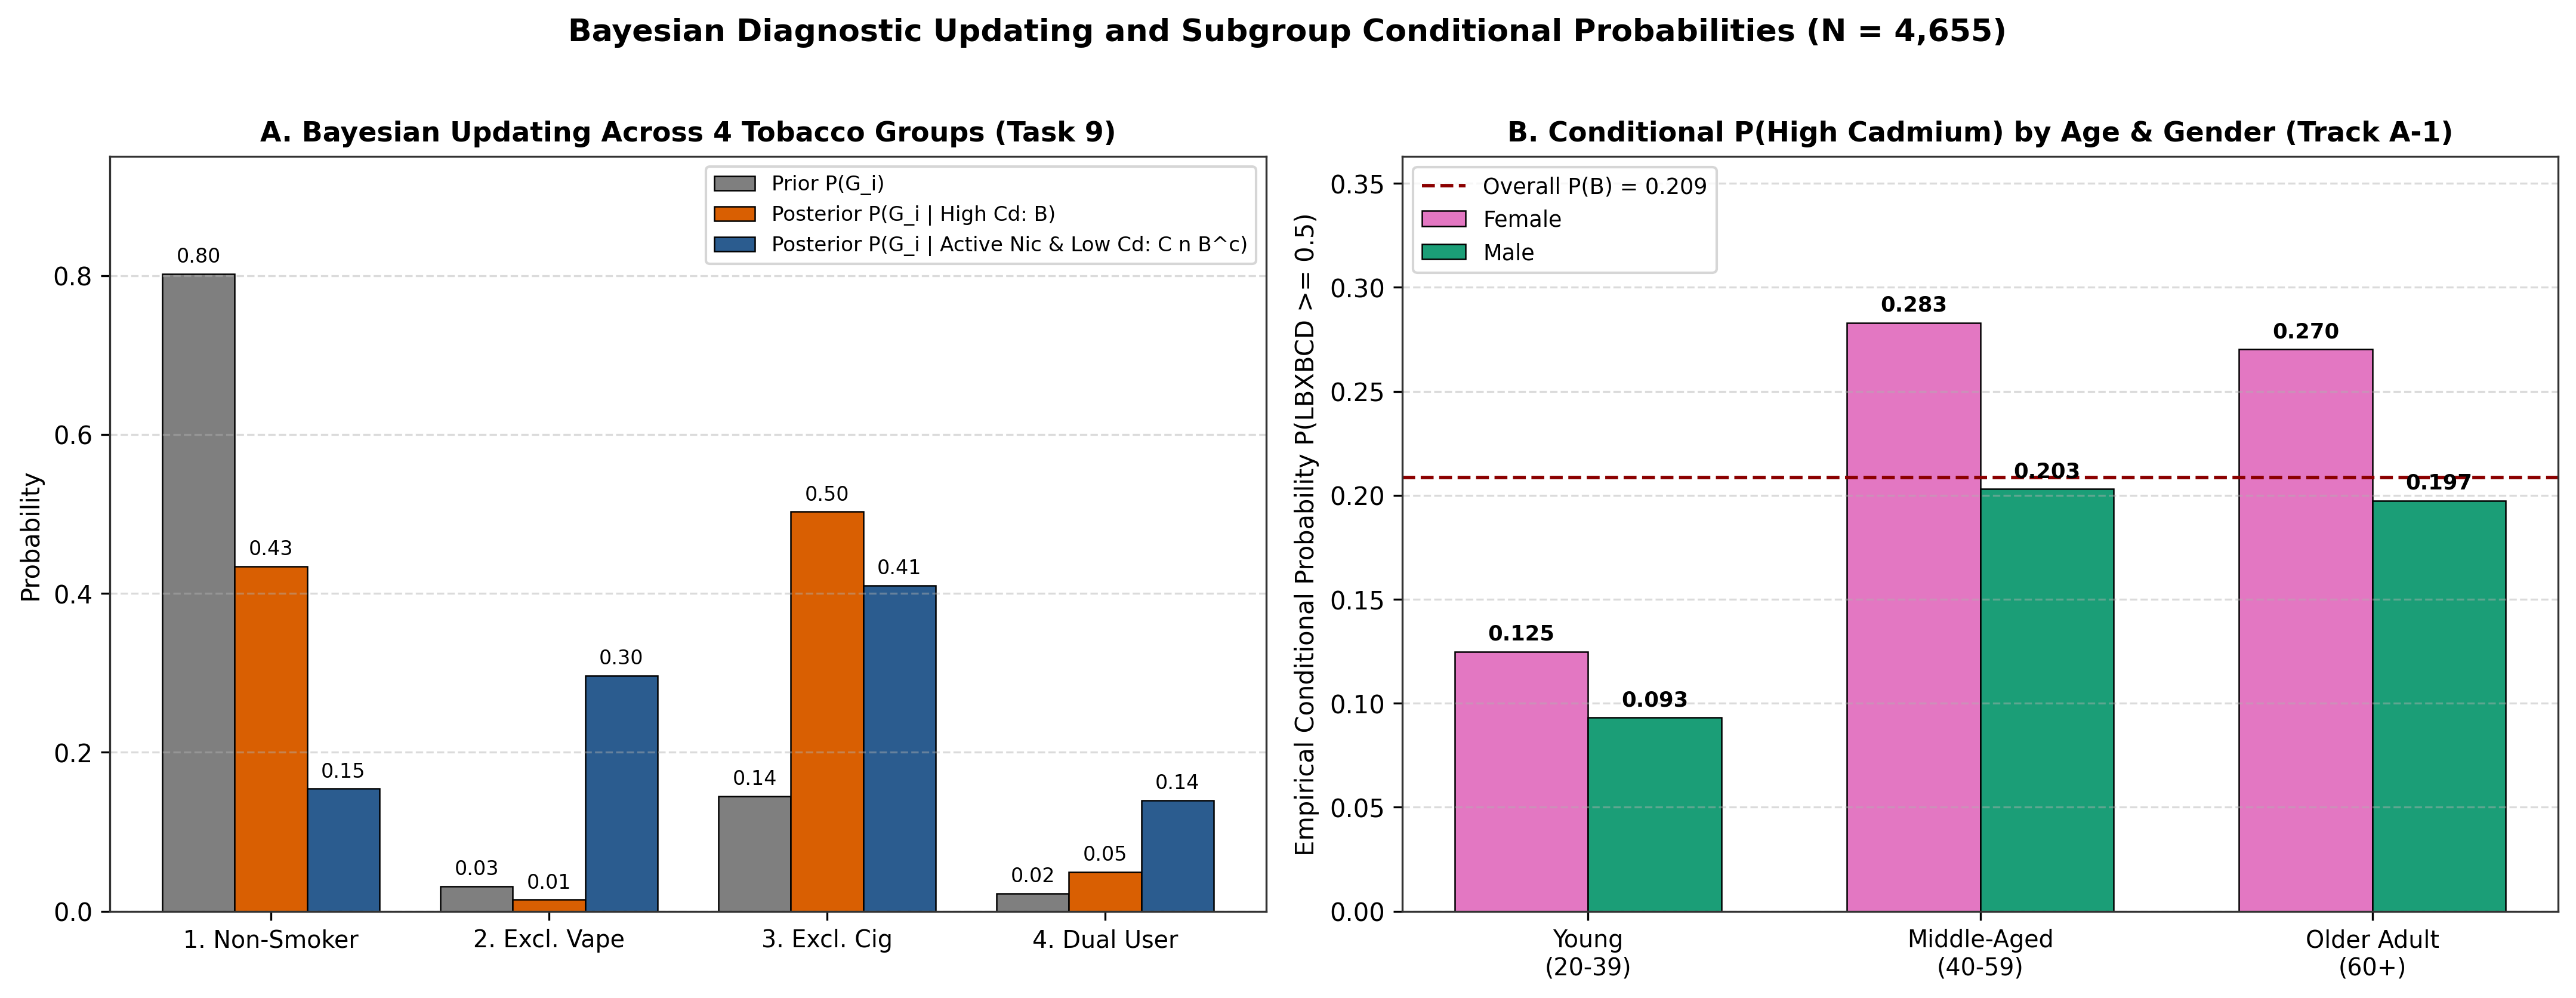
\includegraphics[width=0.80\textwidth]{figures/p2_fig5_bayes_and_subgroups.png}
\caption{به‌روزرسانی بیزی احتمال چهار گروه مصرف تحت دو شواهد زیستی (الف) و احتمال شرطی کادمیوم بالای خون در تقاطع رده‌های سنی و جنسیت (ب).}
\end{figure}


\section{الزام الف-۲: مدل دوجمله‌ای برای شمارش در زیرنمونه‌های هم‌اندازه}

برای آزمون تجربی برازش مدل دوجمله‌ای و اثر خوشه‌بندی (بدون استفاده از بازنمونه‌گیری با جایگذاری یا \lr{Bootstrap})، جمعیت تحلیلی (\lr{$N = 4,655$}) را به \lr{155} زیرنمونه مجزا و هم‌اندازه با حجم \lr{$n = 30$} نفر افراز کردیم (\lr{4,650} مشاهده با کنار گذاشتن \lr{5} مشاهده باقی‌مانده) و شمارش افراد دارای کادمیوم بالا ($B$) را در دو شیوه افراز «تصادفی» (با بذر \lr{42}) و «خوشه‌ای» (مرتب‌شده بر اساس \lr{SDMVSTRA} و \lr{SDMVPSU}) با توزیع نظری $\text{Binomial}(30, 0.2086)$ مقایسه نمودیم.

\begin{table}[htbp]
\centering
\caption{مقایسه مشخصات توزیع تجربی شمارش کادمیوم بالا در \lr{155} زیرنمونه مجزای \lr{30} نفری با مدل نظری $\text{Binomial}(30, 0.2086)$}
\resizebox{\textwidth}{!}{
\begin{tabular}{lllllllll}
\toprule
توزیع مورد مقایسه & تعداد زیرنمونه ($M$) & میانگین & واریانس & انحراف معیار & نسبت پراکندگی ($\text{Var} / \text{Var}_{\text{theo}}$) & کمینه & میانه & بیشینه \\
\midrule
مدل نظری $\text{Binomial}(30, 0.2086)$ & \lr{155} & \lr{6.258} & \lr{4.952} & \lr{2.225} & \lr{1.00} & \lr{0} & \lr{6.0} & \lr{30} \\
تجربی: افراز تصادفی (\lr{Random}) & \lr{155} & \lr{6.258} & \lr{4.751} & \lr{2.180} & \lr{0.96} & \lr{2} & \lr{6.0} & \lr{15} \\
تجربی: افراز خوشه‌ای (\lr{PSU-Ordered}) & \lr{155} & \lr{6.265} & \lr{5.741} & \lr{2.396} & \lr{1.16} & \lr{1} & \lr{6.0} & \lr{15} \\
\bottomrule
\end{tabular}
}
\end{table}

\begin{table}[htbp]
\centering
\caption{مقایسه فراوانی و احتمال تجربی بازه‌های شمارش ($k$) در دو شیوه افراز با پیش‌بینی مدل دوجمله‌ای}
\resizebox{0.92\textwidth}{!}{
\begin{tabular}{lllllll}
\toprule
بازه شمارش ($k$ از \lr{30}) & احتمال نظری دوجمله‌ای & تعداد مورد انتظار (از \lr{155}) & مشاهده تصادفی & احتمال تصادفی & مشاهده خوشه‌ای & احتمال خوشه‌ای \\
\midrule
\lr{0} تا \lr{3} نفر & \lr{0.1016} & \lr{15.7} & \lr{14} & \lr{0.0903} & \lr{15} & \lr{0.0968} \\
\lr{4} تا \lr{5} نفر & \lr{0.2807} & \lr{43.5} & \lr{45} & \lr{0.2903} & \lr{45} & \lr{0.2903} \\
\lr{6} تا \lr{7} نفر & \lr{0.3393} & \lr{52.6} & \lr{58} & \lr{0.3742} & \lr{56} & \lr{0.3613} \\
\lr{8} تا \lr{9} نفر & \lr{0.2007} & \lr{31.1} & \lr{24} & \lr{0.1548} & \lr{25} & \lr{0.1613} \\
\lr{10} نفر و بیشتر & \lr{0.0777} & \lr{12.0} & \lr{14} & \lr{0.0903} & \lr{14} & \lr{0.0903} \\
\bottomrule
\end{tabular}
}
\end{table}

نتایج جداول و شکل \lr{6} پیش‌بینی نظری تسک \lr{5} را به صورت تجربی تایید می‌کنند. میانگین (\lr{6.258} و \lr{6.265}) و میانه (\lr{6.0}) در هر دو شیوه دقیقاً هم‌تراز با مدل نظری است، اما رفتار واریانس متمایز است: در افراز تصادفی (پنل \lr{A}) که ساختار خوشه‌ای از بین رفته است، واریانس تجربی (\lr{4.751}) تطابق نزدیکی با واریانس دوجمله‌ای (\lr{4.952}، نسبت \lr{0.96}) دارد. اما در افراز خوشه‌ای \lr{PSU} (پنل \lr{B})، واریانس تجربی به \lr{5.741} افزایش می‌یابد که بیانگر \lr{16\%} بیش‌پراکندگی (\lr{Overdispersion}) نسبت به مدل دوجمله‌ای و \lr{21\%} پراکندگی بیشتر نسبت به افراز تصادفی در اثر همبستگی درون‌خوشه‌ای \lr{NHANES} است.

\begin{figure}[htbp]
\centering
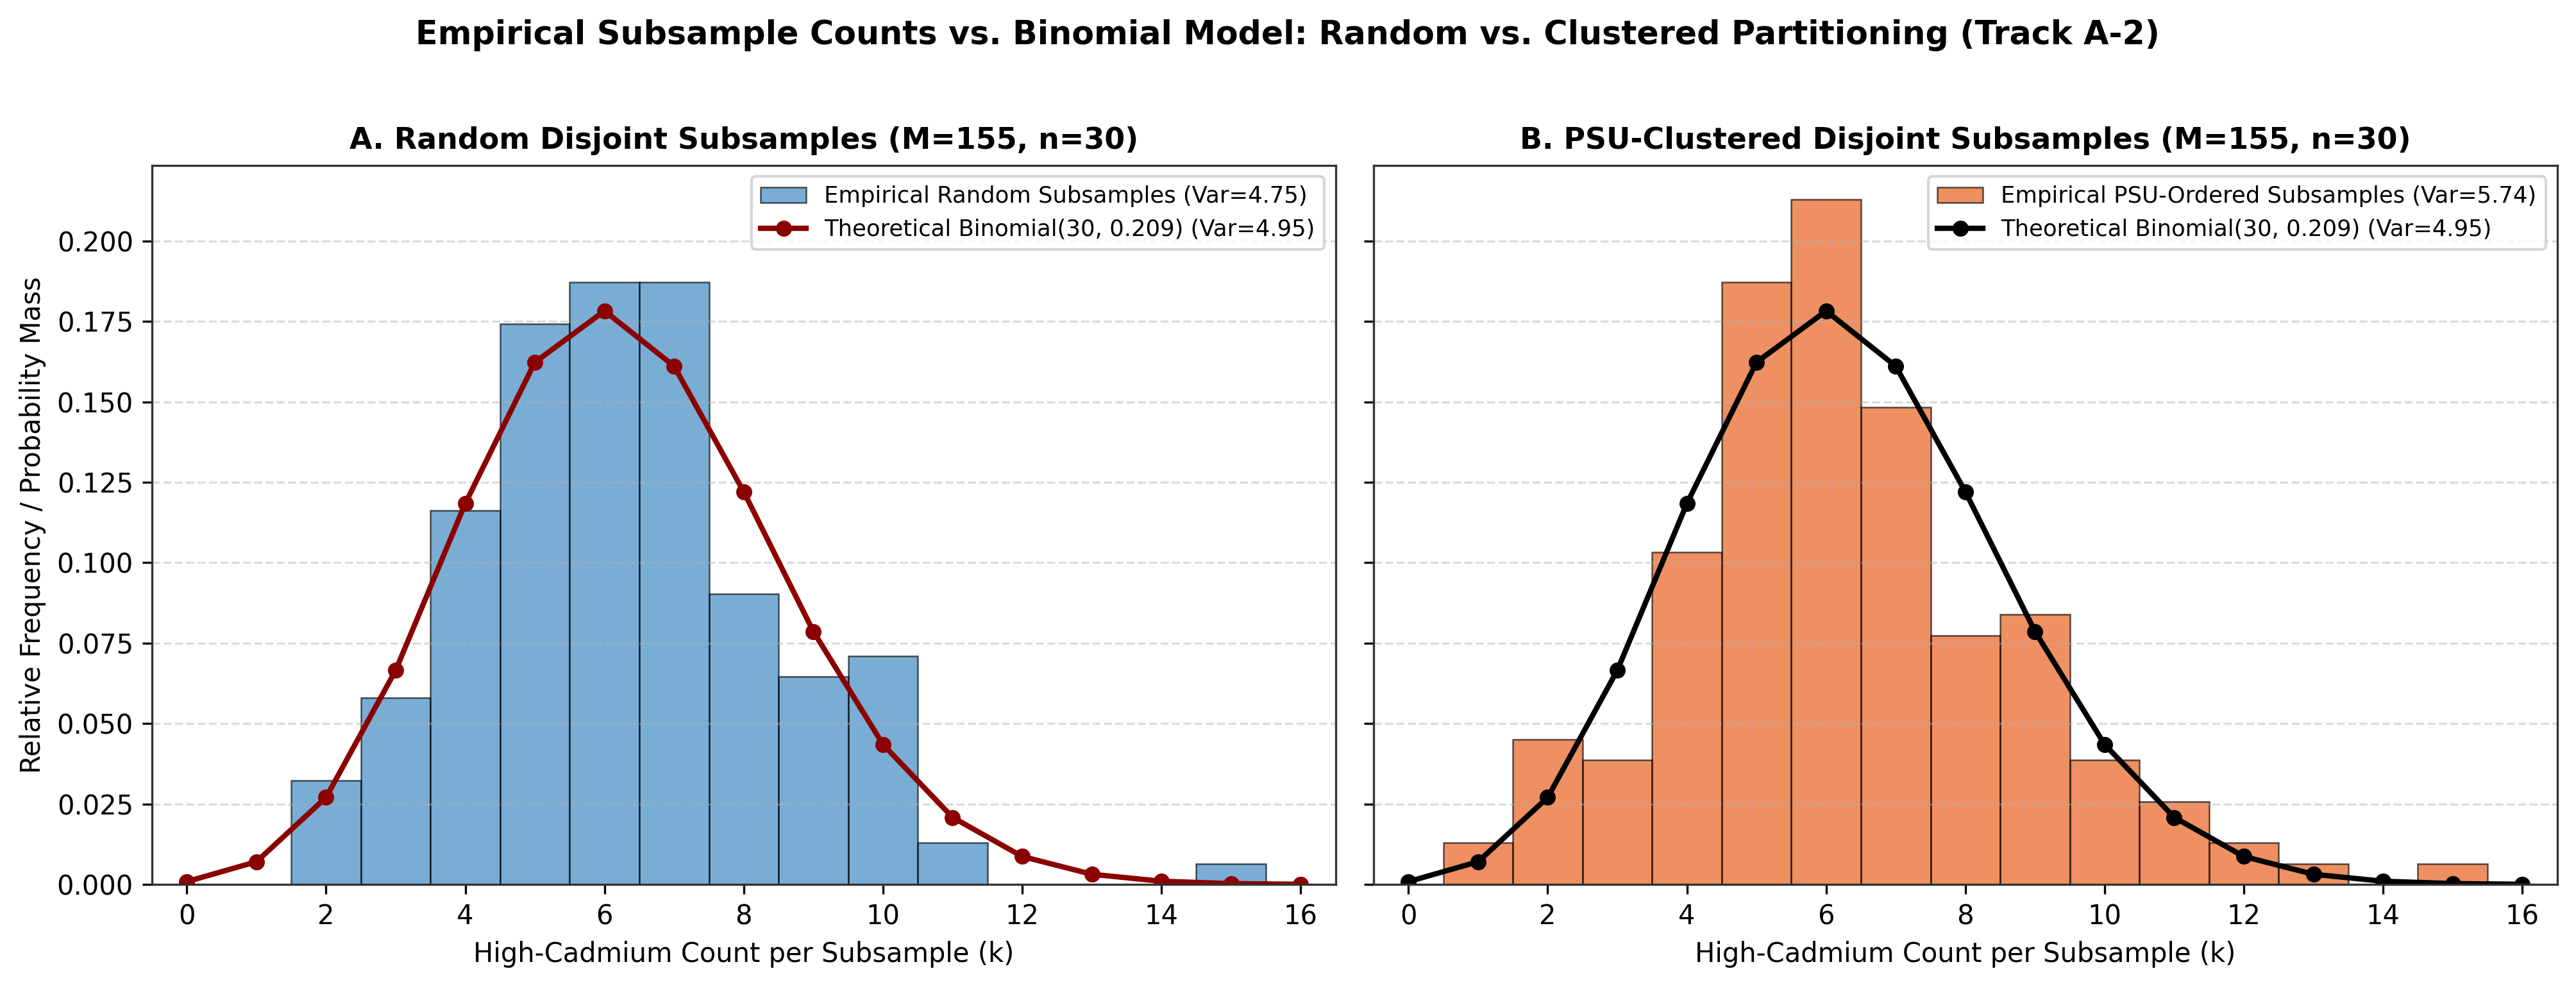
\includegraphics[width=0.80\textwidth]{figures/p2_fig6_binomial_subsamples.png}
\caption{مقایسه توزیع تجربی شمارش کادمیوم بالا در \lr{155} زیرنمونه مجزای \lr{30} نفری با منحنی نظری دوجمله‌ای در حالت افراز تصادفی (الف) و افراز خوشه‌ای \lr{PSU} (ب).}
\end{figure}


\section{الزام الف-۳: شکل توزیع، نقاط دورافتاده و تقریب نرمال هموگلوبین خون}

به عنوان یک شاخص بالینی سلامت مجزا از کادمیوم، غلظت هموگلوبین خون کامل ($Y_3 = \text{LBXHGB}$ بر حسب \lr{g/dL}) را بر روی \lr{4,638} مشاهده معتبر جمعیت تحلیلی (\lr{2,555} زن و \lr{2,083} مرد) از نظر چولگی، کشیدگی، نقاط دورافتاده توکی (\lr{$1.5 \times \text{IQR}$}) و تقریب نرمال تحلیل می‌کنیم.

\begin{table}[htbp]
\centering
\caption{پروفایل چولگی، کشیدگی، قانون تجربی و نقاط دورافتاده توکی (\lr{$1.5 \times \text{IQR}$}) برای هموگلوبین خون (\lr{LBXHGB})}
\resizebox{\textwidth}{!}{
\begin{tabular}{llllllllllllll}
\toprule
جمعیت & $N$ & میانگین & میانه & \lr{SD} & \lr{IQR} & چولگی & کشیدگی مازاد & درون $1\text{SD}$ & درون $2\text{SD}$ & مرزهای توکی & پرت چپ & پرت راست & کل پرت (\lr{\%}) \\
\midrule
کل جمعیت تحلیلی & \lr{4,638} & \lr{13.909} & \lr{13.9} & \lr{1.450} & \lr{1.9} & \lr{-0.329} & \lr{0.807} & \lr{69.84\%} & \lr{95.45\%} & \lr{[10.15, 17.75]} & \lr{53} & \lr{12} & \lr{65} (\lr{1.40\%}) \\
فقط زنان & \lr{2,555} & \lr{13.245} & \lr{13.3} & \lr{1.201} & \lr{1.5} & \lr{-0.683} & \lr{1.604} & \lr{72.60\%} & \lr{95.23\%} & \lr{[10.25, 16.25]} & \lr{45} & \lr{8} & \lr{53} (\lr{2.07\%}) \\
فقط مردان & \lr{2,083} & \lr{14.723} & \lr{14.8} & \lr{1.308} & \lr{1.5} & \lr{-0.725} & \lr{2.140} & \lr{72.35\%} & \lr{94.38\%} & \lr{[11.75, 17.75]} & \lr{58} & \lr{12} & \lr{70} (\lr{3.36\%}) \\
\bottomrule
\end{tabular}
}
\end{table}

\begin{table}[htbp]
\centering
\caption{مقایسه صدک‌های تجربی هموگلوبین خون در کل جمعیت تحلیلی (\lr{$N = 4,638$}) با صدک‌های نظری $N(13.909, 1.450^2)$}
\resizebox{0.88\textwidth}{!}{
\begin{tabular}{llllllll}
\toprule
شاخص صدک & \lr{P1} & \lr{P5} & \lr{P25} & \lr{P50} & \lr{P75} & \lr{P95} & \lr{P99} \\
\midrule
مقدار تجربی (\lr{g/dL}) & \lr{10.000} & \lr{11.500} & \lr{13.000} & \lr{13.900} & \lr{14.900} & \lr{16.200} & \lr{17.200} \\
مقدار نظری نرمال (\lr{g/dL}) & \lr{10.535} & \lr{11.524} & \lr{12.931} & \lr{13.909} & \lr{14.888} & \lr{16.295} & \lr{17.283} \\
اختلاف (تجربی $-$ نظری) & \lr{-0.535} & \lr{-0.024} & \lr{+0.069} & \lr{-0.009} & \lr{+0.012} & \lr{-0.095} & \lr{-0.083} \\
\bottomrule
\end{tabular}
}
\end{table}

تقریب نرمال $N(13.909, 1.450^2)$ برای بدنه اصلی هموگلوبین خون برازش بسیار خوبی دارد (شکل \lr{7}): میانگین (\lr{13.909}) و میانه (\lr{13.900}) تقریباً یکسان‌اند، نسبت مشاهدات درون یک، دو و سه انحراف معیار (\lr{69.84\%}، \lr{95.45\%} و \lr{99.31\%}) منطبق بر قانون تجربی است و از صدک \lr{P5} تا \lr{P99} حداکثر اختلاف صدک‌های تجربی با نظری کمتر از \lr{0.10 g/dL} است.

با این حال، دو ظرافت بالینی در توزیع دیده می‌شود. نخست، از مجموع \lr{65} نقطه دورافتاده توکی (\lr{1.40\%}، بیرون از \lr{[10.15, 17.75]} در پنل \lr{C})، \lr{53} مورد در دنباله چپ (شامل \lr{3} مورد کم‌خونی بسیار شدید زیر \lr{$3 \times \text{IQR}$} تا کمینه \lr{6.60 g/dL}) و تنها \lr{12} مورد در دنباله راست قرار دارند که علت اصلی چولگی منفی خفیف (\lr{-0.329}) و انحراف انتهای چپ نمودار \lr{Q-Q} (پنل \lr{B}، صدک \lr{P1} برابر \lr{10.0} در برابر \lr{10.535} نظری) است. دوم، تفکیک جنسیتی (پنل \lr{D}) نشان می‌دهد که توزیع کل مخلوطی از دو توزیع با اختلاف میانگین \lr{1.48 g/dL} است (زنان \lr{13.245} با \lr{$\text{SD}=1.201$} و مردان \lr{14.723} با \lr{$\text{SD}=1.308$}). همین ترکیب دو قله باعث کاهش ظاهری چولگی و کشیدگی در کل نمونه نسبت به درون هر جنس به تنهایی (چولگی \lr{-0.683} در زنان و \lr{-0.725} در مردان) شده است؛ لذا در تحلیل‌های دقیق بالینی، تفکیک جنسیت و توجه به دنباله کم‌خونی ضروری است.

\begin{figure}[htbp]
\centering
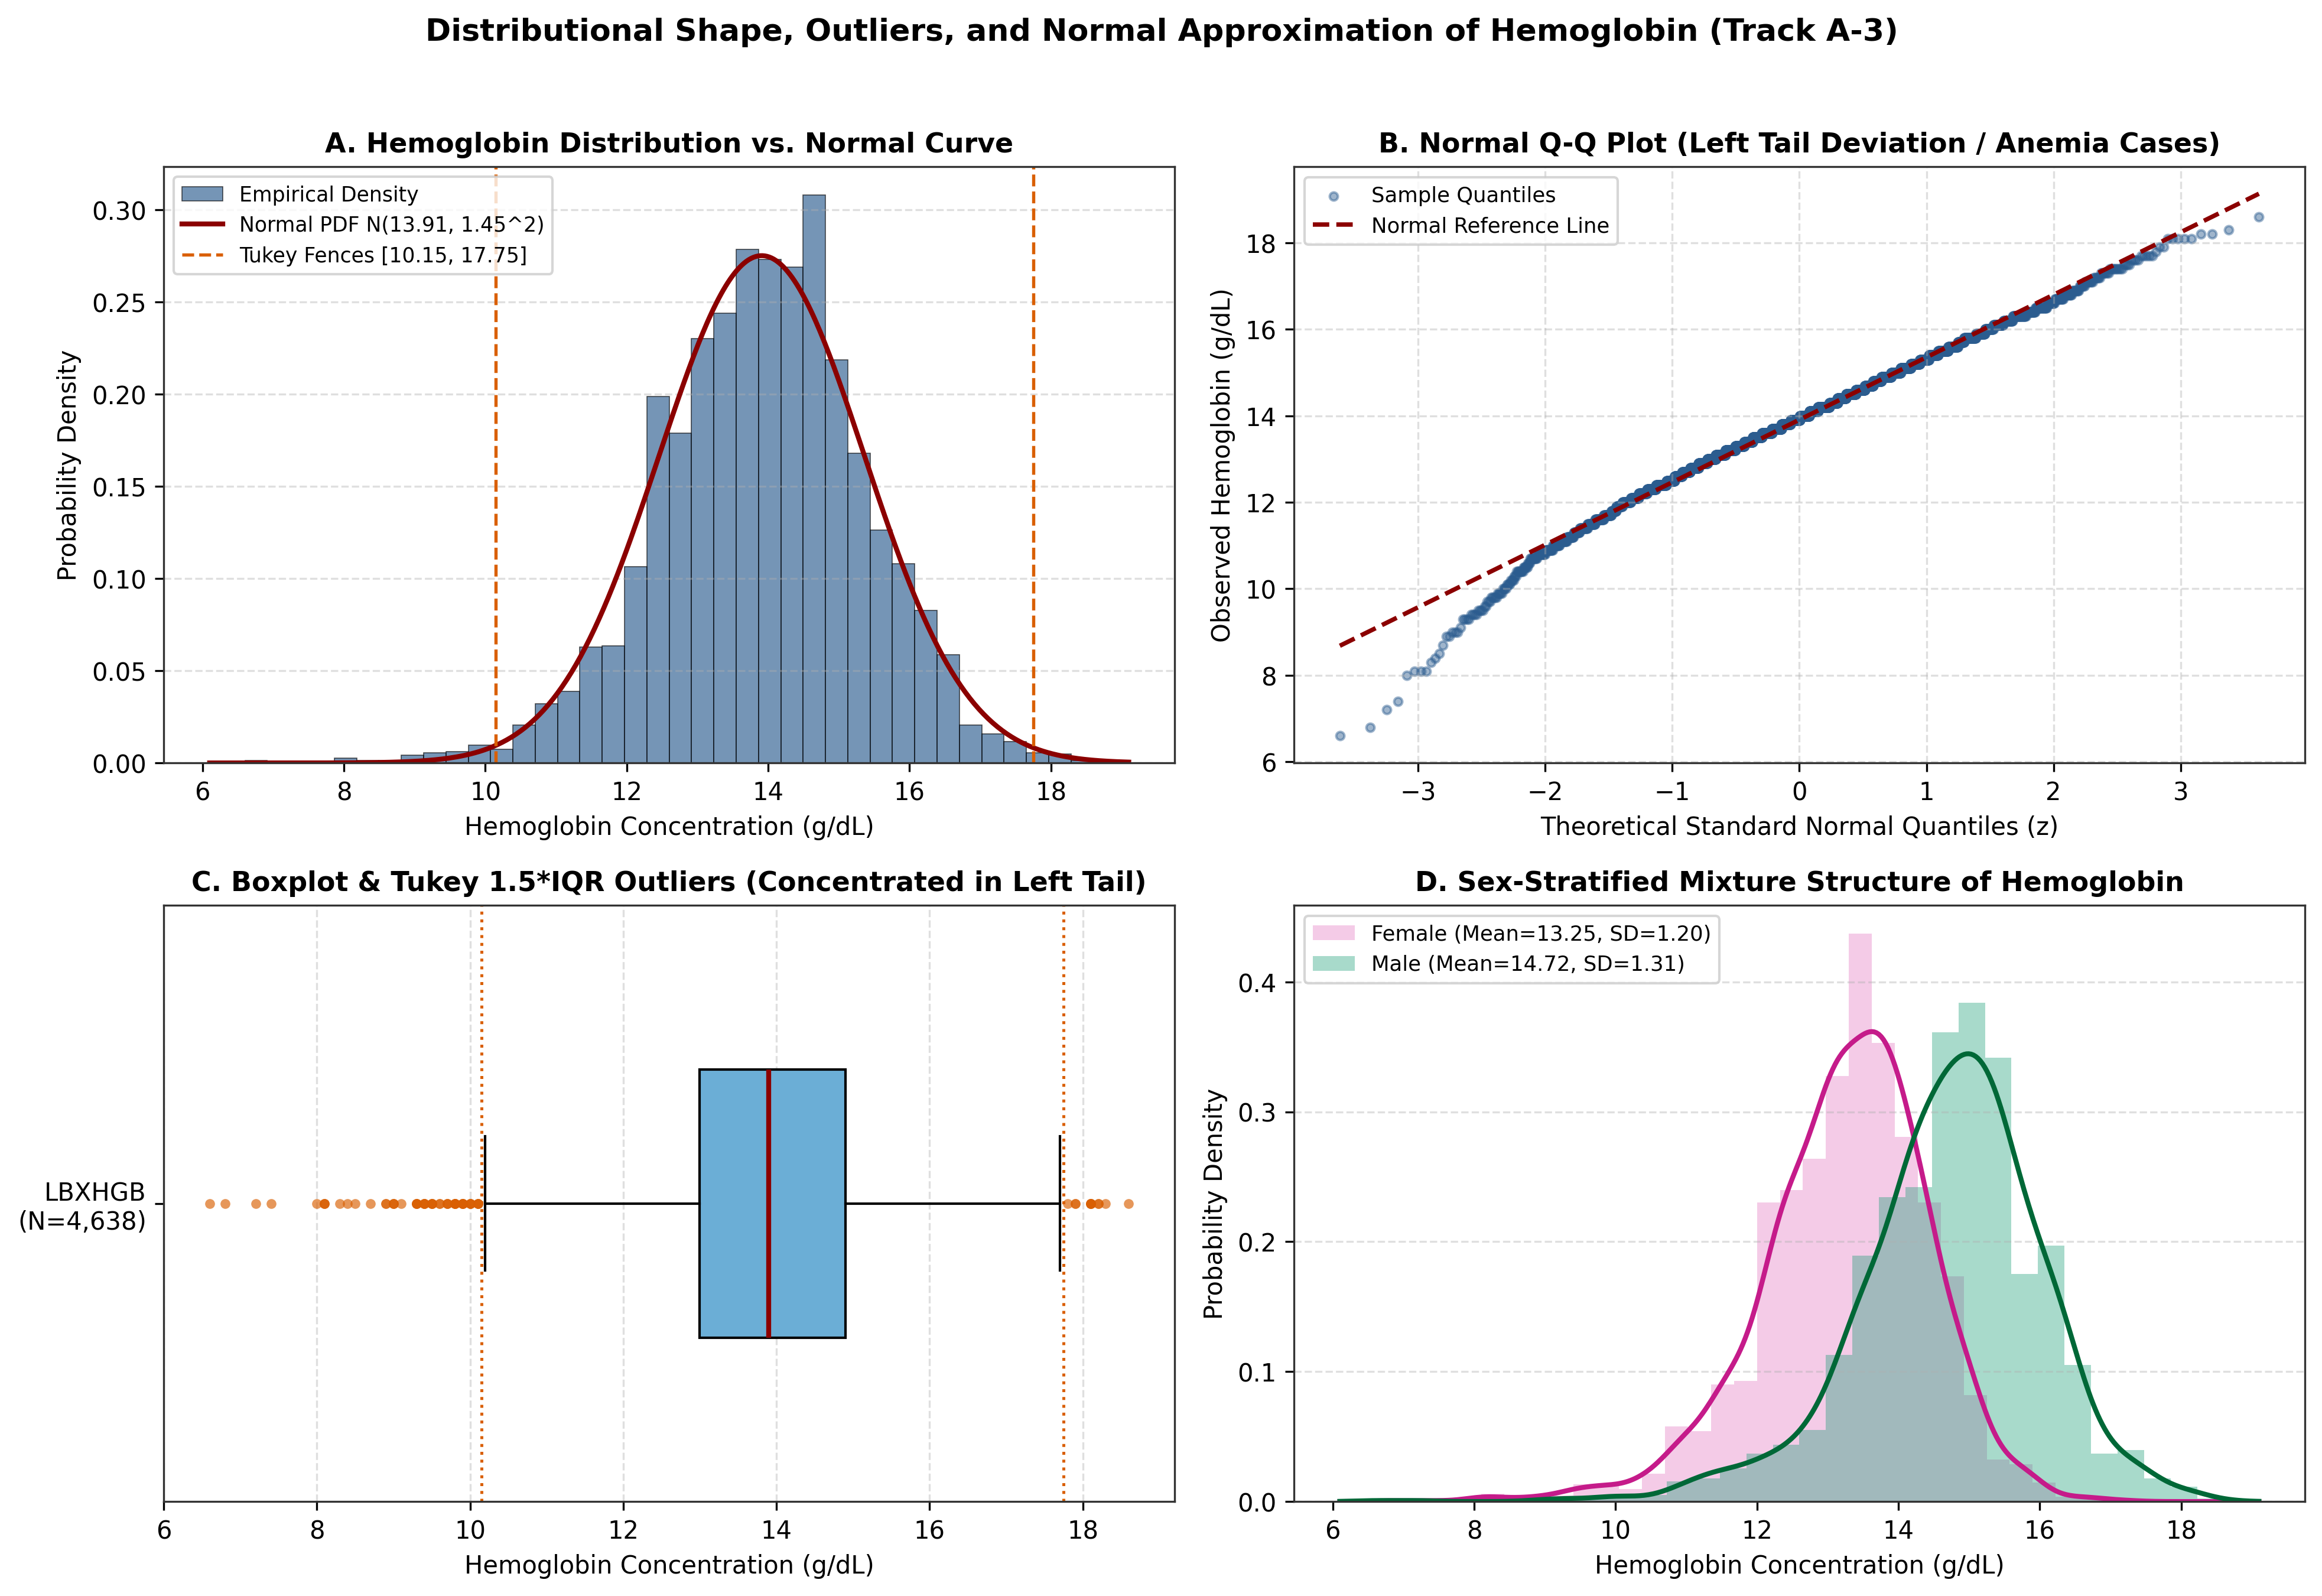
\includegraphics[width=0.74\textwidth]{figures/p2_fig7_hemoglobin_shape.png}
\caption{ارزیابی شکل توزیع هموگلوبین خون (\lr{LBXHGB}): هیستوگرام و منحنی نرمال (الف)، نمودار \lr{Q-Q} (ب)، نمودار جعبه‌ای نقاط دورافتاده (ج) و ساختار مخلوط دو جنس (د).}
\end{figure}


\section{الزام الف-۴: نقش وزن‌های نمونه‌گیری در احتمال تجربی}

فراوانی نسبی خام در نمونه ($\hat{p}_{\text{unw}} = \frac{1}{N}\sum_{i=1}^{N} I_E(\omega_i)$) تنها در نمونه‌گیری تصادفی ساده با شانس انتخاب برابر و نرخ پاسخ یکسان، برآوردگر بی‌تورش احتمال در جمعیت است. در \lr{NHANES}، برای برآورد احتمال واقعی وقوع رویداد در جمعیت بزرگسال ایالات متحده، هر فرد باید متناسب با وزن خون‌گیری خود (\lr{WTPH2YR}) وزن بگیرد: $\hat{p}_{\text{weighted}}(E) = \frac{\sum_{i=1}^{N} w_i \, I_E(\omega_i)}{\sum_{i=1}^{N} w_i}$. جدول زیر نسخه خام و وزن‌دار را برای رویدادهای حاشیه‌ای و احتمال شرطی $P(B \mid G_i)$ مقایسه می‌کند.

\begin{table}[htbp]
\centering
\caption{مقایسه فراوانی نسبی خام نمونه با برآورد احتمال در جمعیت (وزن \lr{WTPH2YR}) برای رویدادهای حاشیه‌ای و شرطی}
\resizebox{\textwidth}{!}{
\begin{tabular}{llllll}
\toprule
بخش / رویداد مورد بررسی & تعداد در نمونه & فراوانی خام (نمونه) & احتمال وزن‌دار (جمعیت) & اختلاف (وزن‌دار $-$ خام) & تغییر نسبی (\lr{\%}) \\
\midrule
$B$: کادمیوم بالای خون (\lr{LBXBCD $\ge 0.5$}) & \lr{971} & \lr{0.2086} & \lr{0.1856} & \lr{-0.0230} & \lr{-11.02\%} \\
$A$: سیگار احتراقی ($G_3 \cup G_4$) & \lr{775} & \lr{0.1665} & \lr{0.1672} & \lr{+0.0007} & \lr{+0.43\%} \\
$C$: نیکوتین فعال (\lr{LBXCOT $\ge 10.0$}) & \lr{912} & \lr{0.1959} & \lr{0.2014} & \lr{+0.0055} & \lr{+2.79\%} \\
$G_2$: مصرف‌کننده انحصاری ویپ & \lr{146} & \lr{0.0314} & \lr{0.0386} & \lr{+0.0073} & \lr{+23.19\%} \\
سالمندان \lr{60} سال به بالا (عامل طراحی نمونه) & \lr{2,178} & \lr{0.4679} & \lr{0.3182} & \lr{-0.1497} & \lr{-31.99\%} \\
\midrule
شرطی $P(B \mid G_1)$: غیرسیگاری (\lr{Non-Smoker}) & \lr{3,734} & \lr{0.1127} & \lr{0.0941} & \lr{-0.0186} & \lr{-16.54\%} \\
شرطی $P(B \mid G_2)$: انحصاری ویپ (\lr{Excl. Vape}) & \lr{146} & \lr{0.0959} & \lr{0.0727} & \lr{-0.0232} & \lr{-24.15\%} \\
شرطی $P(B \mid G_3)$: انحصاری سیگار (\lr{Excl. Cig}) & \lr{672} & \lr{0.7262} & \lr{0.6990} & \lr{-0.0272} & \lr{-3.75\%} \\
شرطی $P(B \mid G_4)$: مصرف دوگانه (\lr{Dual User}) & \lr{103} & \lr{0.4660} & \lr{0.3759} & \lr{-0.0901} & \lr{-19.33\%} \\
\bottomrule
\end{tabular}
}
\end{table}

دلیل شکاف میان فراوانی خام نمونه و برآورد احتمال در جمعیت، ترکیب انتخاب \lr{100\%} سالمندان \lr{60+} سال درون خانوارها در چرخه \lr{2021-2023} با نرخ پاسخ متفاوت زیرگروه‌ها در خون‌گیری است. همان‌طور که در جدول دیده می‌شود، سهم سالمندان از \lr{46.79\%} در نمونه خام به سهم واقعی \lr{31.82\%} در جامعه (\lr{-31.99\%} تغییر نسبی) تعدیل می‌شود. در نتیجه، چون کادمیوم با سن انباشته می‌شود، فراوانی خام کادمیوم بالا (\lr{0.2086}) نسبت به احتمال واقعی جمعیتی آن (\lr{0.1856}) بیش از \lr{11\%} بیش‌برآورد شده بود. در جهت عکس، به دلیل جوان‌تر بودن ویپرها، احتمال جمعیتی مصرف انحصاری ویپ با \lr{23.19\%} افزایش نسبی به \lr{0.0386} و نیکوتین فعال به \lr{0.2014} می‌رسد، در حالی که احتمال سیگار احتراقی ($A$) تقریباً ثابت می‌ماند (\lr{+0.43\%}) زیرا کاهش سهم سیگاری‌های انحصاری مسن‌تر و افزایش سهم مصرف‌کنندگان دوگانه جوان‌تر همدیگر را خنثی می‌کنند. در نهایت، پس از وزن‌دهی، احتمال شرطی کادمیوم بالا در هر چهار گروه کاهش می‌یابد و شکاف میان سیگار انحصاری و انحصاری ویپ حتی شدیدتر می‌شود: نسبت $P(B \mid G_3)$ به $P(B \mid G_2)$ از \lr{7.57} برابر در نمونه خام به \lr{9.61} برابر در برآورد جمعیتی (\lr{0.6990} در برابر \lr{0.0727}) افزایش می‌یابد.

\end{document}
